\subsection{Conjugacy Theorems}

THEOREM 2. --- Let B be a semisimple ring and Z its center; suppose that B is a finitely generated Z-module. Let A be a right Artinian ring, and let f and g be ring homomorphisms from B to A; write \(f_{Z}\) and \(g_{Z}\) for the restrictions of f and g to Z. The following properties are equivalent:

\begin{enumerate}
\def\labelenumi{(\roman{enumi})}
\item
  There exists an inner automorphism \(\theta\) of A such that \(g = \theta \circ f\) .
\item
  There exists an inner automorphism \(\theta\) of A such that \(g_{\mathbb{Z}} = \theta \circ f_{\mathbb{Z}}\) .
\end{enumerate}

Since the ring A is right Artinian, \(A_{d}\) is a right A-module of finite length (VIII, p.~6, Theorem 1). Hence \(A^{f}\) and \(A^{g}\) are (B, A)-bimodules of finite length. By Lemma 1 (VIII, p.~254), assertion (i) means that \(A^{f}\) and \(A^{g}\) are isomorphic (B, A)-bimodules and assertion (ii) that they are isomorphic (Z, A)-bimodules. The equivalence of (i) and (ii) therefore follows from Lemma 2 (VIII, p.~254).

COROLLARY. --- Let A and B be algebras over the field K. Suppose that B is central simple and of finite degree and that A is right Artinian. Let f and g be K-algebra homomorphisms from B to A. There exists an inner automorphism \(\theta\) of A such that \(g = \theta \circ f\) .

In the notation of Theorem 2, we have \(\mathrm{Z} = \mathrm{K}\) and therefore \(f_{\mathrm{Z}} = 1_{\mathrm{Z}} = g_{\mathrm{Z}}\) .

THEOREM 3 (Skolem-Noether). --- Let A and B be simple K-algebras and Z(A) and Z(B) their centers. Suppose that the algebra B has finite degree over K and that the algebra \(Z(A) \otimes_{K} Z(B)\) is a field (which is, in particular, the case when A or B is central). Let f and g be K-algebra homomorphisms from B to A. There exists an inner automorphism \(\theta\) of A such that \(g = \theta \circ f\) .

By Lemma 1 of VIII, p.~254, it suffices to prove that the (B,A)-bimodules \(A^{f}\) and \(A^{g}\) are isomorphic. Now, we can view \(A^{f}\) and \(A^{g}\) as left modules over the algebra \(C = B \otimes_{K} A^{o}\) , which is simple by Proposition 7 of VIII, p.~221. As right A-modules, \(A^{f}\) and \(A^{g}\) are isomorphic to \(A_{d}\) , hence have finite length because the ring A is simple (VIII, p.~121, Corollary 1). A fortiori, \(A^{f}\) and \(A^{g}\) are C-modules of finite length. Let S be a simple C-module; there exist strictly positive integers m and n such that \(A^{f}\) is isomorphic to \(S^{m}\) and \(A^{g}\) to \(S^{n}\) . The right A-module S therefore has nonzero finite length. Since the right A-modules underlying \(A^{f}\) and \(A^{g}\) are isomorphic, they have the same length; we therefore have m = n, so that the C-modules \(A^{f}\) and \(A^{g}\) are isomorphic.

COROLLARY 1. --- Let A be a central simple algebra over K, and let L be an extension of K of finite degree. If f and g are K-algebra homomorphisms from L to A, then there exists an inner automorphism \(\theta\) of A such that \(g = \theta \circ f\) .

COROLLARY 2. --- Let A be a central simple algebra over K, and let L be a subalgebra of A that is a field. Every K-algebra homomorphism from L to A extends to an inner automorphism of A.

COROLLARY 3. --- Let D be a field of finite degree over K with center K. Every element of D is algebraic over K. Let x and y be elements of D; there exists an element a of \(D^{*}\) such that \(y = axa^{-1}\) if and only if x and y have the same minimal polynomial over K.

The first assertion follows from Corollary 1 of V, §3, No.~1, p.~17.

Suppose that there exists an element \(a\) of \(\mathrm{D}^*\) such that \(y = axa^{-1}\) ; for every polynomial \(\mathrm{P}\) of \(\mathrm{K}[\mathrm{X}]\) , we have \(\mathrm{P}(y) = a\mathrm{P}(x)a^{-1}\) , and, in particular, we have \(\mathrm{P}(x) = 0\) if and and only if \(\mathrm{P}(y) = 0\) . Consequently, \(x\) and \(y\) have the same minimal polynomial over \(\mathrm{K}\) (V, §3, No.~1, p.~16, Theorem 1).

Conversely, suppose that x and y have the same minimal polynomial. By loc. cit., there exists a K-isomorphism u from K{[}x{]} to K{[}y{]} such that \(u(x) = y\) , and K{[}x{]} is a field. By Corollary 2, u extends to an inner automorphism \(\theta : z \mapsto aza^{-1}\) of D, and we therefore have \(y = \theta(x) = axa^{-1}\) .

PROPOSITION 1. --- Let A be a central simple algebra of finite degree over K. Let B be a K-algebra, and let f and g be algebra homomorphisms from B to A. The following properties are equivalent:

\begin{enumerate}
\def\labelenumi{(\roman{enumi})}
\item
  There exists an inner automorphism \(\theta\) of A such that \(g = \theta \circ f\) .
\item
  As left B-modules, \(\mathrm{A}^f\) and \(\mathrm{A}^g\) are isomorphic.
\end{enumerate}

By Lemma 1 (VIII, p.~254), property (i) is equivalent to the fact that \(A^{f}\) and \(A^{g}\) are isomorphic as (B, A)-bimodules. Since A is finite-dimensional over K, \(A^{f}\) and \(A^{g}\) are B-modules of finite length. Since the center of A is equal to K, the equivalence of (i) and (ii) follows from Lemma 2 of VIII, p.~254 applied to the \((\mathrm{A}^{\circ}, \mathrm{B}^{\circ})\) -bimodules \(A^{f}\) and \(A^{g}\) .

\subsection{Automorphisms of Semisimple Algebras}

THEOREM 4. --- Let A be a semisimple ring, Z its center, and u an automorphism of A. Suppose that A is a finitely generated Z-module and that we have \(u(z) = z\) for every z in Z. Then u is an inner automorphism.

This follows from Theorem 2 of VIII, p.~256 applied with \(f = \mathrm{Id}_{\mathrm{A}}\) and \(g = u\) .

Example. --- Theorem 4 applies in the following two specific cases:

\pandocbounded{
\includegraphics[keepaspectratio]{images/part002_1d1a6ca2.jpg}}

\begin{enumerate}
\def\labelenumi{\alph{enumi})}
\item
  Let D be a field and Z its center. If D has finite degree over Z, then every automorphism of D that fixes the elements of Z is an inner automorphism. The assumption that D has finite degree over Z is essential (VIII, p.~269, Exercise 4).
\item
  Let V be a finite-dimensional vector space over the field K. Every automorphism of the K-algebra \(\operatorname{End}_{\mathrm{K}}(\mathrm{V})\) is an inner automorphism; this result extends to the case when the space V is not finite-dimensional over K (VIII, p.~272, Exercise 13).
\end{enumerate}

In particular, every automorphism of a matrix algebra \(\mathbf{M}_{n}(\mathrm{K})\) (with \(n \geqslant 1\) ) is an inner automorphism. This result admits the following generalization.

PROPOSITION 2. --- Let L be a commutative ring and V a free L-module of finite dimension m. Suppose that every L-module M such that \(M^{m}\) is isomorphic to \(L^{m}\) is isomorphic to L. Then every automorphism of the L-algebra \(\operatorname{End}_{\mathrm{L}}(\mathrm{V})\) is an inner automorphism.

Set \(B = \text{End}_{\text{L}}(\text{V})\) . Let u be an automorphism of the L-algebra B. We view V as a left B-module; let \(u_{*}(\text{V})\) be the left B-module associated with u, with external law \((b, v) \mapsto u(b)(v)\) (II, §1, No.~13, p.~221). Let \((e_1, \ldots, e_m)\) be a basis of the L-module V; given elements \(v_1, \ldots, v_m\) of V, there exists a unique element b of B such that we have \(b(e_i) = v_i\) for \(1 \leqslant i \leqslant m\) . In other words, the element \(e = (e_1, \ldots, e_m)\) of \(V^m\) provides a basis of the B-module \(V^m\) . Since u is an automorphism, e also gives a basis of the B-module \(u_{*}(\text{V}^m) = u_{*}(\text{V})^m\) , which is therefore isomorphic to \(V^m\) . The (B,L)-bimodule V is invertible (VIII, p.~102, Example 1). By Theorem 2, b) of VIII, p.~103, there consequently exists an L-module M such that the B-module \(u_{*}(\text{V})\) is isomorphic to \(V \otimes_{L} M\) . The B-modules \(V \otimes_{L} L^m\) and \(V \otimes_{L} M^m\) , respectively isomorphic to \(V^m\) and \(u_{*}(\text{V})^m\) , are therefore isomorphic. By loc. cit., the L-modules \(L^m\) and \(M^m\) are isomorphic. Given the assumption, M is isomorphic to L; consequently, the B-module \(u_{*}(\text{V})\) , which is isomorphic to \(V \otimes_{L} M\) , is isomorphic to V. Let h be a B-module isomorphism from V to \(u_{*}(\text{V})\) ; it is, in particular, an automorphism of the L-module V, that is, an invertible element of B. For b in B and v in V, we have \(h(b(v)) = u(b)(h(v))\) and therefore \(u(b) = hbh^{-1}\) .

The conditions of Proposition 2 are, in particular, satisfied when the commutative ring L is a principal ideal domain (VII, §3, p.~15, Corollary 3) or is Artinian (VIII, p.~37, Theorem 2, d)) or local (VIII, p.~36, Corollary 6).

\subsection{Simple Subalgebras of Simple Algebras}

THEOREM 5. --- Let A be a central simple K-algebra, and let B be a semisimple subalgebra of A of finite degree over K.

\begin{enumerate}
\def\labelenumi{\alph{enumi})}
\item
  The commutant B' of B in A is a simple subalgebra, and B is the commutant of B' in A. Moreover, the algebra \(B \cap B'\) is a semisimple commutative algebra of finite degree over K; it is the common center of B and B'.
\item
  Suppose that B is simple. Then \(B'\) is simple, and we have the equalities
\end{enumerate}

\[
[ \mathrm{A}: \mathrm{B} ^ {\prime} ] _ {s} = [ \mathrm{B}: \mathrm{K} ], \quad [ \mathrm{A}: \mathrm{B} ] _ {s} = [ \mathrm{B} ^ {\prime}: \mathrm{K} ], \quad [ \mathrm{A}: \mathrm{K} ] = [ \mathrm{B}: \mathrm{K} ] [ \mathrm{B} ^ {\prime}: \mathrm{K} ].
\]

(See VIII, p.~124, Definition 2 for the definition of the left degree \([A : B]_s\) .)

The K-algebra \(A^{\circ}\) is central simple, and the K-algebra B is semisimple and of finite degree. By Corollary 1 of VIII, p.~221, the algebra \(C = B \otimes_{K} A^{\circ}\) is semisimple. Let M be the C-module with the same additive group as A and with external law given by the formula \((b \otimes a)a' = ba'a\) for \(a, a'\) in A and b in B. Let u be an element of \(\operatorname{End}_{\mathbf{Z}}(\mathrm{A})\) . Then u belongs to the commutant \(C_{M}'\) of the C-module M if and only if u is right A-linear and left B-linear, in other words, if and only if u belongs to the commutant of \(B_{M}\) in the ring of homotheties of the A-module \(A_{s}\) . We consequently define an isomorphism \(\gamma\) from \(B'\) to \(C_{M}'\) by the relation \(\gamma(b')(x) = b'x\) for \(b'\) in \(B'\) and x in M. Now, the ring C is semisimple, and the C-module M is generated by the element 1 of A. By Proposition 6 of VIII, p.~139, the ring \(C_{M}'\) is semisimple, so the algebra \(B'\) is semisimple.

Let \(\varphi\) be the K-algebra homomorphism from \(A \otimes_K A^\circ\) to \(\mathrm{End}_K(M)\) that sends \(a \otimes a'\) to the K-linear mapping \(x \mapsto axa'\) from M to M. Since the K-algebras A and \(A^\circ\) are central simple, the only two-sided ideals of \(A \otimes_K A^\circ\) are 0 and \(A \otimes_K A^\circ\) (VIII, p.~218, Corollary). We have \(C_M = \varphi(B \otimes A^\circ)\) and \(C_M' = \varphi(B' \otimes K)\) . The homomorphism \(\varphi\) is not zero; it is therefore injective. Since the ring C is semisimple, we have \(C_M'' = C_M\) by Proposition 5 of VIII, p.~139. It follows that the subalgebra \(B \otimes_K A^\circ\) of \(A \otimes_K A^\circ\) is the commutant of the subalgebra \(B' \otimes_K K\) . The commutant of \(B' \otimes_K K\) in \(A \otimes_K K\) is therefore equal to \((B \otimes_K A^\circ) \cap (A \otimes_K K)\) , that is, to \(B \otimes K\) by Proposition 19 of II, §7, No.~9, p.~311. Hence the commutant of \(B'\) in A is equal to B. The algebra \(L = B \cap B'\) is the center of B. Since B is a semisimple algebra of finite degree over K, the algebra L is commutative and semisimple and has finite degree over K. Since B is the commutant of \(B'\) in A, the center of \(B'\) is also equal to \(L = B \cap B'\) (VIII, p.~77). We have proved a).

Now suppose that the algebra B is simple. By Corollary 2 of VIII, p.~222, the ring C is simple. By Proposition 4 of VIII, p.~123 applied to the C-module M, whose commutant is isomorphic to \(B'\) , the ring \(B'\) is simple and M is a \(B'\) -module of finite length. In other words, \(B'\) is a simple subring of the simple ring A, and the left degree \([A : B']_{s}\) is an integer \(m \geqslant 1\) . Viewed as a left \(B'\) -module, A has a finite basis \((a_{1}, \ldots, a_{m})\) . Moreover (loc. cit.), \(\varphi\) induces by restriction an isomorphism from C to \(\mathrm{C}_{\mathrm{M}}'' = \mathrm{End}_{\mathrm{B}'}(\mathrm{A})\) , and the mapping \(c \mapsto (ca_{1}, \ldots, ca_{m})\) from C to \(A^{m}\) is therefore bijective. Consequently, C is a free right A-module of dimension m. Now, we have \(C = B \otimes A^{o}\) , so C is a free right A-module of dimension {[}B : K{]}; it follows that \([A : B']_{s} = m = [B : K]\) . From Proposition 6 of VIII, p.~125, we deduce

\[
[ \mathrm{A}: \mathrm{K} ] = [ \mathrm{A}: \mathrm{B} ^ {\prime} ] _ {s} [ \mathrm{B} ^ {\prime}: \mathrm{K} ] = [ \mathrm{B}: \mathrm{K} ] [ \mathrm{B} ^ {\prime}: \mathrm{K} ];
\]

since we also have

\[
[ \mathrm{A}: \mathrm{K} ] = [ \mathrm{A}: \mathrm{B} ] _ {s} [ \mathrm{B}: \mathrm{K} ]
\]

and \([B:K]\) is finite and nonzero, we conclude that we have the equality \([A:B]_{s}=[B^{\prime}:K]\) (Set Theory, III, §6, No.~3, p.~188, Corollary 3). We have proved b).

\pandocbounded{
\includegraphics[keepaspectratio]{images/part002_69e19a74.jpg}}

Let A be a central simple K-algebra of finite degree. There can exist semisimple commutative subalgebras B of A satisfying \([A:K]\neq[B:K][B':K]\) (Exercise 1 of VIII, p.~269).

THEOREM 6. --- Let A be a central simple K-algebra, B a subalgebra of A of finite degree, and B' its commutant in A.

\begin{enumerate}
\def\labelenumi{\alph{enumi})}
\item
  Suppose that B is central simple. Then \(B'\) is central simple, and the K-algebra homomorphism \(\theta : B \otimes_{K} B' \to A\) that sends \(b \otimes b'\) to \(bb'\) is an isomorphism.
\item
  Suppose that B is semisimple, and let \(L = B \cap B'\) . Then \(B'\) is a semisimple algebra. The commutant \(L'\) of L in A is a semisimple ring with center L, and the ring homomorphism \(\psi : B \otimes_{L} B' \to L'\) that sends \(b \otimes b'\) to \(bb'\) is an isomorphism.
\end{enumerate}

Let us prove a). If B is central simple, then \(B'\) is central simple by Theorem 5 of VIII, p.~259. Hence the K-algebra \(B \otimes_{K} B'\) is simple (VIII, p.~222, Corollary 2), and the homomorphism \(\theta : B \otimes_{K} B' \to A\) is injective. Now, by the equality of \([A : B']_{s}\) and \([B : K]\) (Theorem 5), the left \(B'\) -modules \(B \otimes_{K} B'\) and A are free of the same finite dimension; they are therefore \(B'\) -modules of the same finite length. By Corollary 2 of II, §1, No.~10, p.~213, \(\theta\) is bijective.

Let us prove b). By Theorem 5, the algebra L is commutative, of finite degree over K, and semisimple. By loc. cit. applied to L, its commutant \(L'\) in A is a semisimple algebra, and L is the commutant of \(L'\) in A, so L is the center of \(L'\) . Since L is the center of the semisimple rings \(L'\) , B, and \(B'\) , we can identify \(L'\) with a finite product of simple rings \(L_{i}'\) (for \(i \in I\) ), so that we have

\[
\mathrm{L} = \prod_ {i \in \mathrm{I}} \mathrm{L} _ {i}, \qquad \mathrm{B} = \prod_ {i \in \mathrm{I}} \mathrm{B} _ {i}, \qquad \mathrm{B} ^ {\prime} = \prod_ {i \in \mathrm{I}} \mathrm{B} _ {i} ^ {\prime},
\]

where \(L_{i}\) is the center of \(L_{i}^{\prime}\) and where \(B_{i}\) and \(B_{i}^{\prime}\) are subalgebras of \(L_{i}^{\prime}\) with center \(L_{i}\) that are each other's commutants in \(L_{i}^{\prime}\) . We view \(L_{i}^{\prime}\) as a central simple algebra over the commutative field \(L_{i}\) and \(B_{i}\) as a central simple \(L_{i}\) -algebra of finite degree. By assertion a), the canonical mapping \(\psi_{i}: B_{i} \otimes_{L_{i}} B_{i}^{\prime} \to L_{i}^{\prime}\) that sends \(b_{i} \otimes b_{i}^{\prime}\) to \(b_{i}b_{i}^{\prime}\) is a ring isomorphism. Now, we can identify \(B \otimes_{L} B^{\prime}\) with \(\prod_{i \in I}(B_{i} \otimes_{L_{i}} B_{i}^{\prime})\) , so that \(\psi\) is the product of the family of mappings \((\psi_{i})_{i \in I}\) . Therefore, \(\psi\) is a ring isomorphism.

COROLLARY. --- Suppose that the field K is algebraically closed and that A is a simple algebra of finite degree over K. Let B be a simple subalgebra of A, and let B' be the commutant of B in A. Then B' is a simple K-algebra, B is the commutant of B', we have \([A:K]=[B:K][B':K]\) , and the canonical homomorphism from \(B\otimes_{K}B'\) to A is a K-algebra isomorphism.

Since every simple algebra of finite degree over \(K\) is central, the corollary follows from Theorems 5 and 6.

\subsection{Maximal Commutative Subalgebras}

We say that a subalgebra of a K-algebra A is a maximal commutative subalgebra of A if it is a maximal element of the set of commutative subalgebras of A.

Lemma 3. --- Let A be a K-algebra and L a subalgebra of A.

\begin{enumerate}
\def\labelenumi{\alph{enumi})}
\item
  The algebra \(\mathrm{L}\) is a maximal commutative subalgebra of \(\mathrm{A}\) if and only if \(\mathrm{L}\) is equal to its commutant \(\mathrm{L}'\) in \(\mathrm{A}\) .
\item
  Let \(\mathrm{K}'\) be a nonzero commutative K-algebra. Then \(\mathrm{L}\) is a maximal commutative subalgebra of A if and only if \(\mathrm{L}_{(\mathrm{K}')}\) is a maximal commutative subalgebra of \(\mathrm{A}_{(\mathrm{K}')}\) .
\end{enumerate}

Let us prove a). First suppose that L is equal to \(L'\) . Then L is commutative; if M is a commutative subalgebra of A containing L, then we have \(xy = yx\) for \(x\) in \(\mathrm{L}\) and \(y\) in \(\mathrm{M}\) , so \(\mathrm{M} \subset \mathrm{L}'\) and therefore \(\mathrm{M} = \mathrm{L}\) . Consequently, \(\mathrm{L}\) is a maximal commutative subalgebra of \(\mathrm{A}\) .

Conversely, suppose that L is a maximal commutative subalgebra of A, and let x be an element of \(L'\) . The subalgebra M of A generated by \(L \cup \{x\}\) is then commutative and contains L. Because L is maximal, we have M = L, and so \(x \in L\) and finally \(L = L'\) , which gives a).

By Proposition 6 of III, §4, No.~4, p.~468, the commutant of \(\mathrm{L}_{(\mathrm{K}^{\prime})}\) in \(\mathrm{A}_{(\mathrm{K}^{\prime})}\) is \(\mathrm{L}'_{(\mathrm{K}^{\prime})}\) . Since the equalities \(\mathrm{L} = \mathrm{L}'\) and \(\mathrm{L}_{(\mathrm{K}^{\prime})} = \mathrm{L}'_{(\mathrm{K}^{\prime})}\) are equivalent (II, §7, No.~9, p.~311, Proposition 19), assertion b) follows from a).

PROPOSITION 3. --- Let A be a central simple K-algebra of finite degree, and let L be a semisimple commutative subalgebra of A. The following properties are equivalent:

\begin{enumerate}
\def\labelenumi{(\roman{enumi})}
\item
  The algebra \(\mathrm{L}\) is a maximal commutative subalgebra of \(\mathrm{A}\) .
\item
  The left L-module A is free, of dimension {[}L : K{]}.
\item
  We have \([A:K]=[L:K]^{2}\) .
\end{enumerate}

Suppose, moreover, that A is the algebra \(\operatorname{End}_{\mathrm{K}}(\mathrm{V})\) , where V is a vector space of nonzero finite dimension over K. Then the previous properties are also equivalent to the following:

\begin{enumerate}
\def\labelenumi{(\roman{enumi})}
\setcounter{enumi}{3}
\tightlist
\item
  V is a free L-module of dimension 1.
\end{enumerate}

\begin{enumerate}
\def\labelenumi{\Alph{enumi})}
\tightlist
\item
  Suppose that A is of the form \(\operatorname{End}_{\mathrm{K}}(\mathrm{V})\) , where V is a vector space of nonzero finite dimension over the field K. We will establish the equivalence of conditions (i) through (iv) following the diagram
\end{enumerate}

\[
(i) \Longrightarrow (i v) \Longrightarrow (i i) \Longrightarrow (i i i) \Longrightarrow (i).
\]

Since L is a semisimple commutative algebra of finite degree over K, we can identify it with a finite product \(\prod_{i\in I}L_{i}\) of extensions of K of finite degree (VIII, p.~137, Proposition 3). For every \(i\in I\) , let \(V_{i}\) be the isotypical component of type \(L_{i}\) of the L-module V; it is a vector space of nonzero finite dimension over \(L_{i}\) because V is a faithful L-module (VIII, p.~144, Corollary). We can then identify V with \(\prod_{i\in I}V_{i}\) . Under these conditions, the commutant \(L'\) of L in A, which is simply the algebra \(\operatorname{End}_{\mathrm{L}}(\mathrm{V})\) , can be identified with the product \(\prod_{i\in I}\operatorname{End}_{\mathrm{L}_{i}}(\mathrm{V}_{i})\) .

Suppose that L is a maximal commutative subalgebra of \(\operatorname{End}_{\mathrm{K}}(\mathrm{V})\) . By Lemma 3, a), we have \(L = L'\) , so \(L'\) is commutative and we have \(\dim_{L_i}(V_i) = 1\) for every \(i \in I\) . So (i) implies (iv).

Suppose that the L-module V is free of dimension 1. Let \((e_{1},\ldots,e_{r})\) be a basis of V over K. The mapping \(a\mapsto(ae_{1},\ldots,ae_{r})\) is an isomorphism of left A-modules and therefore of L-modules from A to \(V^{r}\) . Consequently, A is a free left L-module of dimension \(r\) , and we have \(r = \dim_{\mathrm{K}}(\mathrm{V}) = [\mathrm{L}:\mathrm{K}]\) . So (iv) implies (ii).

It is clear that (i) implies (iii).

Finally, suppose that we have \([A:K]=[L:K]^{2}\) , in other words, \(\dim_{\mathrm{K}}(\mathrm{V})=[\mathrm{L}:K]\) . We then have \(\sum_{i}\dim_{\mathrm{L}_{i}}(\mathrm{V}_{i})[\mathrm{L}_{i}:\mathrm{K}]=\sum_{i}[\mathrm{L}_{i}:\mathrm{K}]\) , so that \(V_{i}\) has dimension 1 over \(L_{i}\) for every i. We then have \(\operatorname{End}_{\mathrm{L}_{i}}(\mathrm{V}_{i})=\mathrm{L}_{i}\) for every i, and so \(L^{\prime}=L\) . By Lemma 3, a), L is a maximal commutative subalgebra of A. So (iii) implies (i).

\begin{enumerate}
\def\labelenumi{\Alph{enumi})}
\setcounter{enumi}{1}
\tightlist
\item
  Let us continue with the general case. By Theorem 1 of VIII, p.~252, there exists a separable extension \(\mathrm{K}'\) of \(\mathrm{K}\) of finite degree such that the \(\mathrm{K}'\) -algebra \(\mathrm{A}_{(\mathrm{K}')}\) is isomorphic to an algebra \(\mathrm{End}_{\mathrm{K}'}(\mathrm{V}')\) , where \(\mathrm{V}'\) is a vector space of nonzero finite dimension over \(\mathrm{K}'\) . Then the \(\mathrm{K}'\) -algebra \(\mathrm{L}_{(\mathrm{K}')}\) is commutative and semisimple (VIII, p.~222, Corollary 2). By the first part of the proof, the following properties are equivalent:
\end{enumerate}

(i') The algebra \(L_{(K')}\) is a maximal commutative subalgebra of \(A_{(K')}\) .

(ii') The left \(\mathrm{L}_{(\mathrm{K}^{\prime})}\) -module \(\mathrm{A}_{(\mathrm{K}^{\prime})}\) is free, of dimension \([\mathrm{L}_{(\mathrm{K}^{\prime})}:\mathrm{K}^{\prime}]\) .

(iii') We have \(\left[\mathrm{A}_{\left(\mathrm{K}^{\prime}\right)}:\mathrm{K}^{\prime}\right] = \left[\mathrm{L}_{\left(\mathrm{K}^{\prime}\right)}:\mathrm{K}^{\prime}\right]^{2}\) .

By Lemma 3, b), properties (i) and (i') are equivalent.

Set \(n = [\mathrm{L}:\mathrm{K}]\) ; then \(n = [\mathrm{L}_{(\mathrm{K}^{\prime})}:\mathrm{K}^{\prime}]\) . Property (ii) means that the left L-modules A and \(\mathrm{L}^n\) are isomorphic; by Theorem 3 of VIII, p.~37, this is equivalent to the \(\mathrm{L}_{(\mathrm{K}^{\prime})}\) -modules \(\mathrm{A}_{(\mathrm{K}^{\prime})}\) and \((\mathrm{L}_{(\mathrm{K}^{\prime})})^n\) being isomorphic. The equivalence of (ii) and (ii') follows.

Finally, we have \([A:K]=[A_{(K')}:K']\) and \([L:K]=[L_{(K')}:K']\) , which give the equivalence of properties (iii) and (iii'). We have thus proved the equivalence of properties (i), (ii), and (iii).

COROLLARY. --- Let A be a central simple algebra of finite degree over K, and let L be a semisimple commutative K-algebra such that \([A:K]\) is equal to \([L:K]^{2}\) . Let f and g be injective homomorphisms from L to A. There exists an inner automorphism \(\theta\) of A such that \(g = \theta \circ f\) .

Set \(n = [L : K]\) . Viewed as a left module over the subring \(f(L)\) , A is free of dimension n; this follows from the equivalence of properties (ii) and (iii) of Proposition 3. Since f is an isomorphism from L to \(f(L)\) , the left L-module \(A^{f}\) (whose law of action is given by \((x, a) \mapsto f(x)a\) ) is free of dimension n.~The same holds for \(A^{g}\) , which is therefore isomorphic to \(A^{f}\) . We conclude using the equivalence of properties (i) and (ii) of Proposition 1 (VIII, p.~257).

Suppose that \(\mathbf{A}\) is a central simple algebra of finite degree over \(\mathbf{K}\) .

There can exist maximal commutative subalgebras L of A that are not semisimple and for which \([A:K]\neq[L:K]^{2}\) (VIII, p.~270, Exercise 5).

\subsection{Maximal Étale Subalgebras}

Lemma 4. --- Let A be a central simple algebra of finite degree over K, distinct from K. There exists an étale (V, §6, No.~3, p.~28, Definition 1) subalgebra of A distinct from K.

By Wedderburn's theorem (VIII, p.~120, Theorem 1), we may assume that \(\mathrm{A}\) is of the form \(\mathbf{M}_n(\mathrm{D})\) , where \(n\) is a strictly positive integer and \(\mathrm{D}\) a field with center \(\mathrm{K}\) .

Suppose n \textgreater{} 1. The algebra of diagonal matrices with entries in K is an étale subalgebra of A distinct from K.

Suppose n = 1. Let p be the characteristic exponent of D. By Lemma 1 of VIII, p.~230, there exists an element a of D such that \(a^{p^{m}}\) does not belong to K for any natural number m. So for m sufficiently large, the element \(x = a^{p^{m}}\) is separable over K (V, §7, No.~7, p.~44, Proposition 13), but it does not belong to K. The subalgebra \(\mathrm{K}(x)\) of A is a separable extension of the field K of finite degree, hence an étale subalgebra over K; it is distinct from K.

PROPOSITION 4. --- Let A be a central simple algebra of finite degree over K. Let L be a subalgebra of A, and let L' be the commutant of L in A.

\begin{enumerate}
\def\labelenumi{\alph{enumi})}
\item
  If L is maximal among the semisimple commutative subalgebras of A, then we have \(L = L'\) , and L is a maximal commutative subalgebra of A.
\item
  If L is maximal among the étale subalgebras of A, then we have \(L = L'\) , and L is a maximal commutative subalgebra of A.
\end{enumerate}

We know that the relation \(L = L'\) means that L is a maximal commutative subalgebra of A (VIII, p.~261, Lemma 3, a)). Suppose that L is semisimple, commutative, and distinct from \(L'\) . By Theorem 5 of VIII, p.~259, \(L'\) is semisimple, and L is the commutant of \(L'\) and therefore the center of \(L'\) ; consequently, \(L'\) is not commutative. It suffices to prove that there exists a semisimple commutative subalgebra M of A that is distinct from L and contains L and that is étale if L is étale.

By the structure theorem for semisimple rings (VIII, p.~135, Theorem 1), there exist simple rings \(B_{1},\ldots,B_{r}\) and an isomorphism \(\varphi\) from \(L'\) to \(B_{1}\times\cdots\times B_{r}\) . For \(1\leqslant i\leqslant r\) , denote the center of \(B_{i}\) by \(E_{i}\) ; we then have \(\varphi(\mathrm{L})=\mathrm{E}_{1}\times\cdots\times\mathrm{E}_{r}\) . Since \(L'\) is not commutative, we may assume that \(B_{1}\) , for example, is not commutative; we therefore have \(B_{1}\neq E_{1}\) , and, by Lemma 4, there exists a subalgebra \(M_{1}\) of \(B_{1}\) that is commutative, distinct from \(E_{1}\) , and étale over \(E_{1}\) . Set \(\mathrm{M} = \varphi^{-1}(\mathrm{M}_{1} \times \mathrm{E}_{2} \times \cdots \times \mathrm{E}_{r})\) ; it is a semisimple commutative subalgebra of A containing L and distinct from L. Suppose that L is étale over K; let us prove that M is étale. The extensions \(E_{i}\) of K are separable (V, §6, No.~4, p.~30, Proposition 3). Moreover, since the \(E_{1}\) -algebra \(M_{1}\) and the K-algebra \(E_{1}\) are étale, the K-algebra \(M_{1}\) is also étale (V, §6, No.~5, p.~32, Corollary 2). Thus the K-algebra \(M_{1} \times E_{2} \times \cdots \times E_{r}\) is étale, and therefore so is M.

Let A be a central simple algebra of finite degree over K. A subalgebra of A that is maximal among the semisimple commutative subalgebras of A is called a maximal semisimple commutative subalgebra of A. By Proposition 4, the term ``maximal'' refers to the property of being commutative or of being semisimple and commutative. A subalgebra of A that is maximal among the étale subalgebras of A is called a maximal étale subalgebra of A.

COROLLARY 1. --- Let A be a central simple K-algebra of finite degree. Every semisimple (resp. étale) commutative subalgebra of A is contained in a maximal commutative subalgebra of A that is semisimple (resp. étale).

COROLLARY 2. --- Let D be a field of finite degree over K with center K.

\begin{enumerate}
\def\labelenumi{\alph{enumi})}
\item
  The maximal commutative subfields of D are the maximal commutative subalgebras of D and also the maximal semisimple commutative subalgebras of D. Every commutative subfield L of D is contained in a maximal commutative subfield.
\item
  Let L be a commutative subfield of D that is a separable extension of K; it is contained in a maximal commutative subfield of D that is a separable extension of K.
\item
  Let L be a commutative subfield of D. Then L is a maximal commutative subfield of D if and only if we have \([D:K]=[L:K]^{2}\) .
\end{enumerate}

A subalgebra of D is a field (V, §2, No.~2, p.~10, Proposition 1) and is therefore semisimple. Moreover, a maximal commutative subfield of D contains K. Assertions a) and b) then follow from Corollary 1 and assertion c) of Proposition 3 (VIII, p.~262).

PROPOSITION 5. --- Let A be a central simple algebra of finite degree over K. Let B be a semisimple subalgebra of A, and let B' be the commutant of B.

\begin{enumerate}
\def\labelenumi{\alph{enumi})}
\item
  The algebra B contains a maximal semisimple commutative subalgebra of A if and only if B contains B'.
\item
  Suppose that B contains \(B'\) , and let g be a K-algebra homomorphism from B to A. There exists an inner automorphism \(\theta\) of A that coincides with g on B.
\end{enumerate}

Let L be a maximal commutative subalgebra of A; by Lemma 3 of VIII, p.~261, L is equal to its commutant \(L'\) in A. If B contains L, then its commutant \(B'\) is contained in \(L'\) and therefore in B.

Conversely, suppose that \(B'\) is contained in B. Then \(B'\) is the center of B, and it is a semisimple commutative algebra (VIII, p.~137, Proposition 2). By Corollary 1, there exists a maximal semisimple commutative subalgebra L of A containing \(B'\) . The commutant of L is L (VIII, p.~261, Lemma 3, a)), and that of \(B'\) is equal to B (VIII, p.~259, Theorem 5). The relation \(L \supset B'\) therefore implies \(L \subset B\) . We have proved a).

Let us prove b). Suppose that B contains \(B'\) , and choose a maximal semisimple commutative subalgebra L of A contained in B, which exists by a). Let g be a homomorphism from B to A. By Proposition 3 of VIII, p.~262, we have the equality \([A:K]=[L:K]^{2}\) ; by the corollary of VIII, p.~263, there exists an inner automorphism \(\theta_{1}\) of A that coincides with g on L. If f is the canonical injection of B into A, then the homomorphisms g and \(\theta_{1}\circ f\) have the same restriction to the center \(B'\) of B because \(B'\) is contained in L. By Theorem 2 of VIII, p.~256, there exists an inner automorphism \(\theta\) of A such that \(g=\theta\circ f\) ; in other words, \(\theta\) extends g.

\subsection{Diagonalizable Subalgebras of Simple Algebras}

Let D be a K-algebra that is a field, and let V be a finite-dimensional right vector space over D. Let L be a K-subalgebra of \(\operatorname{End}_{\mathrm{D}}(\mathrm{V})\) that is a diagonalizable K-algebra (V, §6, No.~3, p.~28). By definition, L has finite degree over K, and there exists a basis \((\varepsilon_{i})_{i\in\mathrm{I}}\) of L over K with the following properties:

\[
\varepsilon_ {i} ^ {2} = \varepsilon_ {i}, \varepsilon_ {i} \varepsilon_ {j} = 0 \text { if } i \neq j, \quad \sum_ {i \in I} \varepsilon_ {i} = 1.
\]

Set \(V_{i} = \varepsilon_{i}(V)\) for every i in I; then \((\mathrm{V}_{i})_{i \in \mathrm{I}}\) is a family of nonzero linear subspaces of V with direct sum V (II, §1, No.~8, p.~209, Proposition 12). Let u be an endomorphism of V; then u belongs to L if and and only if for every \(i \in I\) , there exists an element \(\lambda_{i}\) of K such that \(u(x) = \lambda_{i}x\) for every \(x \in V_{i}\) .

Conversely, suppose that V is the direct sum of a family \((\mathrm{V}_{i})_{i\in\mathrm{I}}\) of nonzero linear subspaces. For any element \(\boldsymbol{\lambda}=(\lambda_{i})_{i\in\mathrm{I}}\) of \(K^{I}\) , denote by \(u_{\lambda}\) the endomorphism of the D-vector space V such that \(u_{\boldsymbol{\lambda}}(x)=\lambda_{i}x\) for \(x\in V_{i}\) . The set L of endomorphisms \(u_{\lambda}\) for \(\lambda\in K^{I}\) is a diagonalizable subalgebra of \(\operatorname{End}_{\mathrm{D}}(\mathrm{V})\) having the family \((\varepsilon_{i})_{i\in\mathrm{I}}\) as basis, where \(\varepsilon_{i}\) is the projector with image \(V_{i}\) and kernel \(\sum_{j\neq i}V_{j}\) . We say that L is the diagonalizable subalgebra of \(\operatorname{End}_{\mathrm{D}}(\mathrm{V})\) associated with the direct sum decomposition \(V=\oplus_{i\in\mathrm{I}}V_{i}\) . We have \([L:K]=\operatorname{Card}(I)\leqslant\dim_{\mathrm{D}}(V)\) .

PROPOSITION 6. --- Let L be the diagonalizable subalgebra of \(\operatorname{End}_{\mathrm{D}}(\mathrm{V})\) associated with a direct sum decomposition \(V = \oplus_{i \in I} V_i\) .

\begin{enumerate}
\def\labelenumi{\alph{enumi})}
\item
  The algebra L is maximal among the diagonalizable subalgebras of the K-algebra \(\operatorname{End}_{\mathrm{D}}(\mathrm{V})\) if and only if every \(V_{i}\) has dimension 1 over D.
\item
  The algebra \(\mathrm{L}\) is a maximal commutative subalgebra of \(\operatorname{End}_{\mathrm{D}}(\mathrm{V})\) if and only if we have \(\mathrm{D} = \mathrm{K}\) and every \(\mathrm{V}_i\) has dimension 1 over \(\mathrm{K}\) .
\end{enumerate}

If every vector space \(V_{i}\) has dimension 1 over D, then we have

\[
[ \mathrm{L}: \mathrm{K} ] = \operatorname{Card} (\mathrm{I}) = \dim_ {\mathrm{D}} (\mathrm{V}),
\]

so L is maximal among the diagonalizable subalgebras of \(\operatorname{End}_{\mathrm{D}}(\mathrm{V})\) . In the opposite case, there exists an index \(j \in I\) such that \(\dim_{\mathrm{D}}(\mathrm{V}_{j}) \geqslant 2\) . Choose two nonzero linear subspaces \(V_{j}^{\prime}\) and \(V_{j}^{\prime\prime}\) of \(V_{j}\) with direct sum \(V_{j}\) . The diagonalizable subalgebra of \(\operatorname{End}_{\mathrm{D}}(\mathrm{V})\) associated with the direct sum decomposition \(\mathrm{V} = (\oplus_{i \in \mathbf{I} - \{j\}} \mathrm{V}_{i}) \oplus \mathrm{V}_{j}^{\prime} \oplus \mathrm{V}_{j}^{\prime\prime}\) contains L and is not equal to L; assertion a) follows.

The commutant \(L'\) of L in \(\operatorname{End}_{\mathrm{D}}(\mathrm{V})\) consists of the endomorphisms of the form \((x_{i}) \mapsto (u_{i}(x_{i}))\) , with \((u_{i}) \in \prod_{i \in \mathrm{I}} \operatorname{End}_{\mathrm{D}}(\mathrm{V}_{i})\) . The algebra L is a maximal commutative subalgebra of \(\operatorname{End}_{\mathrm{D}}(\mathrm{V})\) if and only if we have \(L = L'\) (VIII, p.~261, Lemma 3, a)). This relation is therefore equivalent to `` \(\operatorname{End}_{\mathrm{D}}(\mathrm{V}_{i}) = \mathrm{K}\) for every \(i \in I''\) ; assertion b) follows.

PROPOSITION 7. --- Let L be a commutative algebra of finite degree over K. The following properties are equivalent:

\begin{enumerate}
\def\labelenumi{(\roman{enumi})}
\item
  The algebra L is étale.
\item
  There exists a separable extension of K of finite degree that diagonalizes K.
\end{enumerate}

The implication \((\mathrm{ii})\Rightarrow(\mathrm{i})\) follows from V, §6, No.~3, p.~29, Proposition 2. Let us prove the implication \((\mathrm{i})\Rightarrow(\mathrm{ii})\) . Let \(\Omega\) be a separable closure of K. By Theorem 4 of V, §6, No.~7, p.~34, there exist extensions \(L_{1},\ldots,L_{n}\) of K of finite degree, contained in \(\Omega\) , such that L is isomorphic to the product

\(L_{1} \times \cdots \times L_{n}\) . Let N be a Galois extension of K that contains the \(L_{i}\) (V, §10, No.~1, p.~58), and let us prove that \(L_{(N)}\) is diagonalizable. By the primitive element theorem (V, §7, No.~4, p.~40, Theorem 1), for every \(i \in [1, n]\) , there exists an irreducible separable polynomial \(P_{i} \in K[X]\) such that \(L_{i}\) is isomorphic to \(K[X]/(P_{i})\) . Since N is a normal extension of K in which \(P_{i}\) admits a root, the polynomial \(P_{i}\) splits in N{[}X{]}, with simple roots. Consequently, the N-algebra \(L_{i(N)}\) , which is isomorphic to \(N[X]/(P_{i})\) , is isomorphic to \(N^{[L_{i}:K]}\) . Hence \(L_{(N)}\) is diagonalizable.

THEOREM 7. --- Let A be a central simple K-algebra of finite degree and L a subalgebra of A. The following properties are equivalent:

\begin{enumerate}
\def\labelenumi{(\roman{enumi})}
\item
  The algebra L is a maximal étale subalgebra of A.
\item
  There exist an extension \(K'\) of K, an integer \(n \geqslant 1\) , and an isomorphism \(\theta\) from \(\mathrm{A}_{(\mathrm{K}')}\) to \(\mathbf{M}_{n}(\mathrm{K}')\) that sends \(\mathrm{L}_{(\mathrm{K}')}\) to the set of diagonal matrices.
\item
  There exist \(K'\) , n, and \(\theta\) as in (ii), where the extension \(K'\) is, moreover, assumed Galois and of finite degree.
\end{enumerate}

It is clear that (iii) implies (ii).

If property (ii) holds, then \(L_{(K')}\) is a maximal commutative subalgebra of \(A_{(K')}\) (Proposition 6), and it is diagonalizable. The K-algebra L is then étale (V, §6, No.~3, p.~28, Definition 1), and it is a maximal commutative subalgebra of A (VIII, p.~261, Lemma 3, b)). We have proved that (ii) implies (i).

Suppose that property (i) holds. Since L is étale over K, by Proposition 7, there exists a Galois extension \(K_{1}\) of K of finite degree such that the \(K_{1}\) -algebra \(\mathrm{L}_{(\mathrm{K}_{1})}\) is diagonalizable. The algebra A is central simple; by (VIII, p.~252, Theorem 1), there exist a Galois extension \(K_{2}\) , a vector space V of finite dimension n over \(K_{2}\) , and an isomorphism \(\theta\) from \(\mathrm{A}_{(\mathrm{K}_{2})}\) to \(\mathrm{End}_{\mathrm{K}_{2}}(\mathrm{V})\) . By Proposition 1 of V, p.~55, we may assume \(K_{1}=K_{2}\) . By Proposition 4, b) of VIII, p.~264 and Lemma 3, b) of VIII, p.~261, \(\mathrm{L}_{(\mathrm{K}^{\prime})}\) is a maximal commutative subalgebra of \(\mathrm{A}_{(\mathrm{K}^{\prime})}\) , so \(\theta(\mathrm{L}_{(\mathrm{K}^{\prime})})\) is a maximal commutative subalgebra of \(\mathrm{End}_{\mathrm{K}^{\prime}}(\mathrm{V}^{\prime})\) . Let us apply Proposition 6 to the diagonalizable algebra \(\theta(\mathrm{L}_{(\mathrm{K}^{\prime})})\) : there exists a basis \((e_{1},\ldots,e_{n})\) of \(V^{\prime}\) over \(K^{\prime}\) such that \(\theta(\mathrm{L}_{(\mathrm{K}^{\prime})})\) consists of the endomorphisms of \(V^{\prime}\) with diagonal matrix with respect to this basis. So (i) implies (iii).

\BourbakiExercises{Exercises}

\begin{enumerate}
\def\labelenumi{\arabic{enumi})}
\tightlist
\item
  Let \(\mathrm{K}\) be a commutative field, \(\mathrm{A}\) a central simple K-algebra, \(\mathrm{L}\) a semisimple commutative subalgebra of \(\mathrm{A}\) , and \(\mathrm{L}'\) its commutant in \(\mathrm{A}\) .
\end{enumerate}

\begin{enumerate}
\def\labelenumi{\alph{enumi})}
\item
  Suppose that A is the endomorphism algebra of a finite-dimensional K-vector space V. Prove that we have \([L:K][L':K] \geqslant [A:K]\) (cf.~VIII, p.~78, Proposition 1); equality holds if and only if the L-module V is free. Deduce examples where the inequality is strict.
\item
  Prove the inequality \([L:K][L':K] \geqslant [A:K]\) in general.
\end{enumerate}

\begin{enumerate}
\def\labelenumi{\arabic{enumi})}
\setcounter{enumi}{1}
\tightlist
\item
  Let K be a commutative field, A the K-algebra \(\mathbf{M}_{5}(\mathrm{K})\) , B the subalgebra of matrices of the form
\end{enumerate}

\[
\left( \begin{array}{c c c} x & 0 & 0 \\ 0 & Y & 0 \\ 0 & 0 & Y \end{array} \right)  ,
\]

and C the subalgebra of matrices of the form

\[
\left( \begin{array}{c c c c} x & 0 & 0 & 0 \\ 0 & x & 0 & 0 \\ 0 & 0 & x & 0 \\ 0 & 0 & 0 & Y \end{array} \right)  ,
\]

where x runs through K and Y through the algebra \(\mathbf{M}_{2}(\mathrm{K})\) . Prove that B and C are semisimple algebras containing the center Z of A. Then, prove that there exists an isomorphism of K-algebras \(f: B \to C\) that leaves invariant the elements of Z but that there does not exist any automorphism of A extending f (observe that such an automorphism must send a simple component of B to a simple component of C).

¶ 3) a) Let K be a commutative field, A a K-algebra, and B a central simple subalgebra of A of finite rank. Let B' be the commutant of B in A. Prove that the canonical homomorphism from B ⊗K B' to A is bijective. (Note that B and B' are linearly disjoint over K (VIII, p.~225, Exercise 5, d)). Prove, furthermore, that A is the direct sum of a family (M \(_{t}\) ) \(_{t\in I}\) of (B ⊗K B°)-modules isomorphic to B, and observe that for every \(t\in I\) , the element of M \(_{t}\) corresponding to 1 ∈ B by such an isomorphism belongs to B'.)

\begin{enumerate}
\def\labelenumi{\alph{enumi})}
\setcounter{enumi}{1}
\tightlist
\item
  Conversely, let B be a K-algebra such that for every algebra A containing B and having the same unit element as B, the canonical homomorphism from \(B \otimes_{K} B'\) to A is bijective. Prove that the algebra B is central simple and of finite rank (take \(A = \text{End}_{K}(B)\) ; deduce from the assumption that B is central and quasi-simple, and use Exercise 5, e) of VIII, p.~225).
\end{enumerate}

\begin{enumerate}
\def\labelenumi{\arabic{enumi})}
\setcounter{enumi}{3}
\item
  Let \(\mathrm{K}\) be a commutative field, \(\sigma\) an automorphism of \(\mathrm{K}\) distinct from the identity, and \(\mathrm{D}\) the field \(\mathrm{K}((\mathrm{X}))_{\sigma}\) (VIII, p.~19, Exercise 21, e)). Let \(\tau\) be an automorphism of \(\mathrm{K}\) that commutes with \(\sigma\) . Prove that there exists a unique automorphism of \(\mathrm{D}\) extending \(\tau\) and fixing X. Deduce an example of a field automorphism that fixes the center and is not inner.
\item
  Let K be a commutative field, V a vector space of finite dimension n over K, and W a subspace of V distinct from \(\{0\}\) and V. Denote by a the subset of the algebra \(A = \operatorname{End}_{K}(V)\) consisting of the endomorphisms u such that \(\operatorname{Im} u \subset W \subset \operatorname{Ker} u\) and by B the subalgebra \(K + a\) of A. Prove that B is a maximal commutative subalgebra of A, is not semisimple, and has degree possibly \textgreater n over K.
\end{enumerate}

¶ 6) Let D be a field with center K, distinct from K, such that every element of D is algebraic over K.

\begin{enumerate}
\def\labelenumi{\alph{enumi})}
\item
  Prove that D contains a separable commutative extension of degree \(>1\) .
\item
  Let m be an integer; suppose that every element of D has degree \(\leqslant m\) over K. Prove that we have \([D:K]\leqslant m^{2}\) (first prove that D has finite degree using a) and Theorem 5 of VIII, p.~259).
\end{enumerate}

\begin{enumerate}
\def\labelenumi{\arabic{enumi})}
\setcounter{enumi}{6}
\tightlist
\item
  Let A be a commutative ring, M and N A-modules, and \(u: M \to N\) an A-linear mapping. For every maximal ideal m of A, denote by \(u(\mathfrak{m})\) the homomorphism \(M/mM \to N/mN\) induced by u.
\end{enumerate}

\begin{enumerate}
\def\labelenumi{\alph{enumi})}
\item
  Suppose that N is finitely generated and that \(u(\mathfrak{m})\) is surjective for every maximal ideal m of A. Prove that u is surjective (apply Lemma 1 of VIII, p.~81 to the cokernel of u).
\item
  Suppose that M and N are finitely generated, that N is projective, and that \(u(\mathfrak{m})\) is bijective for every maximal ideal m of A. Prove that u is bijective (use the same method).
\item
  Suppose that M and N are projective and finitely generated and that \(u(\mathfrak{m})\) is injective for every maximal ideal m of A. Prove that u induces an isomorphism from M to a direct factor submodule of N (apply a) to the homomorphism \(^{t}u\) .
\item
  Let B be an A-algebra; suppose that the A-module B is faithful, projective, and finitely generated. Prove that A is a direct factor of the A-module B. Prove that if the B-module homomorphism \(u_{(B)} : M_{(B)} \to N_{(B)}\) is bijective, then so is u. Prove that if the B-module \(M_{(B)}\) is projective, then so is the A-module M.
\end{enumerate}

\begin{enumerate}
\def\labelenumi{\arabic{enumi})}
\setcounter{enumi}{7}
\tightlist
\item
  Let A be a commutative ring and S an A-algebra; suppose that S is a projective, faithful, and finitely generated A-module. Denote the A-algebra \(S \otimes_{A} S^{o}\) by E.
\end{enumerate}

\begin{enumerate}
\def\labelenumi{\alph{enumi})}
\tightlist
\item
  Prove that the following conditions are equivalent:
\end{enumerate}

\begin{enumerate}
\def\labelenumi{(\roman{enumi})}
\item
  The (E, A)-bimodule S is invertible.
\item
  The A-algebra S is central, and the E-module S is projective.
\item
  The canonical homomorphism \(E \longrightarrow \operatorname{End}_{\mathrm{A}}(\mathrm{S})\) is bijective.
\item
  For every maximal ideal m of A, the A/m-algebra S/mS is central simple. (Deduce the equivalence of (i), (ii), and (iii) from Theorem 1 of VIII, p.~101 and Corollary 2 of VIII, p.~100 and that of (iii) and (iv) from Theorem 1 of VIII, p.~252 and Exercise 7).
\end{enumerate}

When these conditions are satisfied, we say that \(S\) is an Azumaya algebra over \(A\) .

\begin{enumerate}
\def\labelenumi{\alph{enumi})}
\setcounter{enumi}{1}
\item
  If S and T are Azumaya algebras over A, then so is the A-algebra \(S \otimes_{A} T\) .
\item
  Let B be a commutative A-algebra; if S is an Azumaya algebra over A, then the B-algebra \(S_{(B)}\) is an Azumaya algebra. If the B-algebra \(S_{(B)}\) is an Azumaya algebra and B is a faithful and projective ( \(^{*}\) or faithfully flat \(_{*}\) ) A-algebra, then S is an Azumaya A-algebra (apply Exercise 7, d)).
\end{enumerate}

\begin{enumerate}
\def\labelenumi{\arabic{enumi})}
\setcounter{enumi}{8}
\tightlist
\item
  Let \(\mathrm{A}\) be a commutative ring and \(\mathrm{S}\) an Azumaya A-algebra (Exercise 8).
\end{enumerate}

\begin{enumerate}
\def\labelenumi{\alph{enumi})}
\item
  Prove that the center of S (which we identify with A) is a direct factor of the A-module S (use Exercise 7, d)).
\item
  Let M be an (S,S)-bimodule; denote by \(\mathcal{Z}(M)\) the A-submodule of M consisting of the elements m such that sm = ms for every \(s \in S\) . Deduce from Exercise 8, a) that the canonical homomorphism \(S \otimes_{A} \mathcal{Z}(M) \to M\) is bijective.
\item
  The mapping \(N \mapsto \mathcal{Z}(N)\) is an increasing bijection from the set of \((S, S)\) -sub-bimodules of M to the set of A-submodules of \(\mathcal{Z}(M)\) ; the inverse bijection sends an A-submodule N of \(\mathcal{Z}(M)\) to the \((S, S)\) -sub-bimodule SN of M. In particular, the mapping \(s \mapsto s \cap A\) is an increasing bijection from the set of two-sided ideals of S to the set of ideals of A.
\item
  Let \(\rho : \mathrm{S} \to \mathrm{T}\) be an A-algebra homomorphism, and let \(\mathrm{S}'\) be the commutant of \(\rho(\mathrm{S})\) in T. Prove that the canonical homomorphism \(\mathrm{S} \otimes_{\mathrm{A}} \mathrm{S}' \to \mathrm{T}\) is bijective (apply \(a\) ) to the (S,S)-bimodule T).
\item
  Suppose that every projective A-module L such that \(\dim_{\mathrm{A/m}}(\mathrm{L}/\mathfrak{m}\mathrm{L}) = 1\) for every maximal ideal m of A is free of rank 1 (this is, for example, the case when the ring A is local or a principal ideal domain). Prove that every endomorphism f of the A-algebra S is an inner automorphism (apply a) to the (S,S)-bimodule \(S^{f}\) , using Exercise 8, a) to show that the A-module \(\mathcal{Z}(S^{f})\) is projective).
\end{enumerate}

\begin{enumerate}
\def\labelenumi{\arabic{enumi})}
\setcounter{enumi}{9}
\tightlist
\item
  Let A be a commutative ring and P a faithful, projective, and finitely generated A-module.
\end{enumerate}

\begin{enumerate}
\def\labelenumi{\alph{enumi})}
\item
  Prove that the A-algebra \(\mathrm{S} = \operatorname{End}_{\mathrm{A}}(\mathrm{P})\) is an Azumaya algebra.
\item
  Prove that the left S-module P is projective.
\item
  Let \(P'\) be a second faithful, projective, and finitely generated A-module. Prove that the A-module \(P \otimes_{A} P'\) is faithful, projective, and finitely generated and that the algebra \(\text{End}_{\text{A}}(\text{P} \otimes_{\text{A}} \text{P}')\) can be canonically identified with the algebra \(\text{End}_{\text{A}}(\text{P}) \otimes_{\text{A}} \text{End}_{\text{A}}(\text{P}')\) .
\end{enumerate}

¶ 11) Let A be a commutative integral domain, K its field of fractions, and S an Azumaya A-algebra (Exercise 8).

\begin{enumerate}
\def\labelenumi{\alph{enumi})}
\item
  Prove that the K-algebra \(S_{(K)}\) is central simple. Identify S with a subalgebra of \(S_{(K)}\) .
\item
  Assume from now on that A is the only A-subalgebra of K that is a finitely generated A-module, \(^{*}\) that is, that the ring A is integrally closed, cf.~Comm. Alg., V, §1, No.~1, 2*. Prove that S is maximal (for the inclusion) among the A-subalgebras of \(S_{(K)}\) that are finitely generated as A-modules (apply Exercise 9, d)).
\item
  Suppose, moreover, that A is Noetherian and that the K-algebra \(S_{(K)}\) is isomorphic to \(\operatorname{End}_{\mathrm{K}}(\mathrm{V})\) , where V is a vector space over K. Prove that there exists a finitely generated A-module M without torsion such that the A-algebra S is isomorphic to \(\operatorname{End}_{\mathrm{A}}(\mathrm{M})\) (let x be a nonzero vector of V; take M to be the set of elements \(s(x)\) as s runs through S).
\end{enumerate}

\(^{*}d\) Prove that in the previous construction, we may assume M reflexive (replace M with its bidual). If, moreover, the ring A is regular (AC, X, §4, n° 2, p.~55, définition 1), then the A-module M is projective (apply AC, X, §4, p.~164, exercice 12).*

*¶ 12) Let K be a commutative field, complete for a discrete valuation v (Comm. Alg., VI) that we assume normalized (that is, \(v(\mathrm{K}^{*}) = \mathbf{Z}\) ). Denote the ring of v by A and its residue field by \(\kappa\) . Recall (loc. cit.) that if L is a finite extension of K, then the valuation v admits a unique extension \(v_{L}\) to L; we say that the extension is unramified if \(v_{L}\) has integer values.

\begin{enumerate}
\def\labelenumi{\alph{enumi})}
\item
  Let D be a field with center K; let \(Nrd : D \to K\) be the reduced norm on D (VIII, p.~340, Definition 2). Prove that the mapping \(w_{0} = v \circ Nrd\) is a valuation on D (to prove the inequality \(w_{0}(x + y) \geqslant \inf(w_{0}(x), w_{0}(y))\) , reduce to the case y = 1, and observe that the restriction of \(w_{0}\) to \(K(x)\) is a multiple of \(v_{\mathrm{K}(x)}\) ). Denote by w the normalized valuation on D equivalent to \(w_{0}\) .
\item
  An element x of L is integral over A if and only if we have \(w(x) \geqslant 0\) ; the set of these elements forms a subring B of D.
\item
  Assume from now on that the field \(\kappa\) is perfect. Prove that if D is distinct from K, then it contains an unramified extension of K distinct from K. (In the opposite case, observe that we have \([\kappa_{\mathrm{L}}:\kappa] = 1\) for every extension L of K contained in D. Let \(b\in \mathrm{B}\) , and let \(\pi\) be a uniformizer of D. Apply the previous remark to the field \(\mathrm{K}(b)\) , and prove that \(b\) is in the closure of \(\mathrm{A}(\pi)\) . Since the subspace \(\mathrm{K}(\pi)\) is closed in D (EVT, I, §2, n° 3, p.~14, corollaire 1), we obtain \(\mathrm{B}\subset \mathrm{K}(\pi)\) and finally \(\mathrm{D} = \mathrm{K}(\pi)\) .) d) Prove that there exists a maximal commutative subfield of D that is unramified over K. (Use induction on the reduced degree of D by considering a subfield L of D that is unramified over K and applying the induction hypothesis to the commutant of L in D.)*
\end{enumerate}

\begin{enumerate}
\def\labelenumi{\arabic{enumi})}
\setcounter{enumi}{12}
\tightlist
\item
  Let D be a field, V a left vector space over D, A the ring \(\operatorname{End}_{\mathrm{D}}(\mathrm{V})\) , and f an automorphism of A. Prove that there exist an automorphism \(\sigma\) of D and a bijective mapping \(u: V \to V\) that is semilinear with respect to \(\sigma\) (II, §1, No.~13, p.~223) such that we have \(f(a) = u \circ a \circ u^{-1}\) for every \(a \in A\) . (Let \(V^{f}\) be the A-module with additive group V and external law defined by \((a, v) \mapsto f(a)(v)\) ; deduce from
\end{enumerate}

Proposition 4 of VIII, p.~50 an A-isomorphism \(u: V \to V^{f}\) . Then, observe that \(uDu^{-1}\) is equal to the bicommutant of the D-module V, that is, to D.)

\begin{enumerate}
\def\labelenumi{\arabic{enumi})}
\setcounter{enumi}{13}
\tightlist
\item
  Let D be a field, Z its center, V a left vector space over D, and \(\Omega\) the endomorphism ring of the abelian group V. Endow \(\Omega\) with its natural (D,D)-bimodule structure. Let \(\Gamma\) be the automorphism group of D and \(\Delta\) the subgroup of inner automorphisms (isomorphic to \(D^{*}/Z^{*}\) ).
\end{enumerate}

Let S be a subset of \(\Omega\) consisting of semilinear mappings (relative to an element of \(\Gamma\) ) and F the left D-linear subspace of \(\Omega\) generated by S; it coincides with the right D-linear subspace generated by S.

\begin{enumerate}
\def\labelenumi{\alph{enumi})}
\item
  For \(\theta \in \Gamma / \Delta\) , denote by \(S_{\theta}\) the set of semilinear mappings from V to itself with respect to an automorphism of D belonging to \(\theta\) and by \(F_{\theta}\) the D-linear space of F generated by \(S_{\theta}\) . Prove that F is the direct sum of the subspaces \(F_{\theta}\) for \(\theta \in \Gamma / \Delta\) . b) Prove that if \(S_{\theta}\) is a free subset over Z, then it is also (left and right) free over D (reason as in the proof of Theorem 1 of V, §6, No.~1, p.~27).
\item
  Let E be a (D,D)-sub-bimodule of F. Prove that E is generated (over D) by semilinear mappings belonging to the \(F_{\theta}\) . (Let B be a basis of F contained in S. Prove that E is generated by the vectors \(u \in E\) that have the following property: if \(u = \sum_{i}^{n} \lambda_{i} b_{i}\) with \(\lambda_{i} \neq 0\) and \(b_{i} \in B\) for every i, then the intersection of E and the subspace of F generated by the \(b_{i}\) is reduced to Du. Then deduce from a) that u is semilinear.)
\end{enumerate}

¶ 15) Keep the notation of Exercise 14; denote the ring \(\mathrm{End}_{\mathrm{D}}(\mathrm{V})\) by A. Let G be a group of automorphisms of A and \(\mathrm{G}_0\) the subgroup of elements of G that are inner automorphisms of A. Denote by U(G) the (left and right) D-linear subspace of \(\Omega\) generated by the semilinear bijections \(s\) of V such that the automorphism \(a \mapsto sas^{-1}\) belongs to G, and denote by \(\mathrm{U}_0(\mathrm{G})\) the Z-linear subspace of A generated by the automorphisms \(u\) of V such that the automorphism \(a \mapsto uau^{-1}\) belongs to \(\mathrm{G}_0\) . These are Z-subalgebras of \(\Omega\) .

\begin{enumerate}
\def\labelenumi{\alph{enumi})}
\item
  Let \((s_{\alpha})\) be a basis of \(U_{0}(G)\) over Z consisting of elements of \(S_{0}(G)\) , and let \((g_{\beta})_{\beta\in G/G_{0}}\) be a system of representatives of the classes (mod \(G_{0}\) ) in G. For each \(\beta\in G/G_{0}\) , choose an element \(u_{\beta}\) of \(S(G)\) corresponding to \(g_{\beta}\) . Prove that the elements \(s_{\alpha}u_{\beta}\) form a (left and right) basis of \(U(G)\) over D (use Exercise 14, a)). The degree \([U(G):D]\) is finite if and only if \([U_{0}(G):Z]\) and \((G:G_{0})\) are finite; if this is the case, then we have \([U(G):D]=[U_{0}(G):Z](G:G_{0})\) .
\item
  Prove that \(\mathrm{U}_{0}(\mathrm{G})\) is equal to \(\mathrm{U}(\mathrm{G})\cap\mathrm{A}\) and that \(\mathrm{U}(\mathrm{G}_{0})=\mathrm{D}u_{0}(\mathrm{G})\) is canonically isomorphic to \(\mathrm{U}_{0}(\mathrm{G})\otimes_{\mathrm{Z}}\mathrm{D}\) (use Exercise 14 as well as Exercise 14 of VIII, p.~227). c) An element of \(\mathrm{U}(\mathrm{G})\) is a semilinear mapping from V to itself if and only if it is of the form \(\lambda su_{\beta}\) with \(\lambda\in D\) , \(s\in\mathrm{U}_{0}(\mathrm{G})\) , and \(\beta\in\mathrm{G}/\mathrm{G}_{0}\) (use a), b), and Exercise 14, a)).
\item
  Denote the commutant of U(G) in \(\Omega\) by \(A^{G}\) ; it is the subring of A consisting of the elements invariant under G. Set \(Z^{G} = A^{G} \cap Z\) ; it is the subfield of elements of Z invariant under G. Prove that Z and \(A^{G}\) are linearly disjoint over \(Z^{G}\) (verify that a basis of \(A^{G}\) over \(Z^{G}\) is a free subset of A over Z).
\item
  Prove that if \(U_{0}(G)\) is a simple ring and one of the Z-algebras \(U_{0}(G)\) and D has finite degree, then the ring \(U(G)\) is quasi-simple (deduce from c) that \(U(G_{0})\) is a simple ring, and apply Exercise 14, c) to a two-sided ideal of \(U(G)\) using c)).
\item
  Suppose that V and U(G) are finite-dimensional over D and that the ring \(U_{0}(G)\) is simple. Prove that the ring A{[}G{]} is simple and that we have \([A : A^{G}]_{s} = [U_{0}(G) : Z](G : G_{0})\) (apply Proposition 12 of VIII, p.~205). Prove that the commutant of \(A^{G}\) in \(\Omega\) (resp. in A) is U(G) (resp. \(U_{0}(G)\) ) (use Proposition 5 of VIII, p.~139).
\end{enumerate}

\(g\) ) Deduce that the group of automorphisms of A that fix \(\mathrm{A}^{\mathrm{G}}\) consists of the automorphisms \(a\mapsto vav^{-1}\) , where \(v\) runs through the set of semilinear bijections in \(\mathrm{U(G)}\) . Prove that it is generated by G and the inner automorphisms associated with the invertible elements of \(\mathrm{U_0(G)}\) (use \(c\) ).

\begin{enumerate}
\def\labelenumi{\alph{enumi})}
\setcounter{enumi}{7}
\tightlist
\item
  If \(G = G_{0}\) , then the ring \(A^{G}\) contains Z; prove the converse when D is finite-dimensional over Z (use Theorem 4 of VIII, p.~257).
\end{enumerate}

¶ 16) Keep the notation of Exercise 15, and suppose, moreover, that V is finite-dimensional over D. A subring B of A is called weakly Galois (resp. Galois) in A if its commutant B' in Ω is generated as a (left or right) D-vector space by semilinear mappings (resp. bijections) from V to itself. Denote by DB the subring of Ω generated by D and B.

\begin{enumerate}
\def\labelenumi{\alph{enumi})}
\item
  Prove that if B is simple and weakly Galois, then V is a semisimple module of finite length over DB. (Let W be an isotypical component of the B-module V and S a simple DB-submodule of W. Let \(\Sigma\) be the set of semilinear mappings v belonging to \(B'\) . Observe that \(v(\mathrm{S})\) is an DB-module for \(v \in \Sigma\) and deduce from Corollary 3 of VIII, p.~56 that W is contained in the sum of the \(v(\mathrm{S})\) for \(v \in \Sigma\) .)
\item
  Suppose that the ring B is simple and weakly Galois and that its commutant \(B_{0}^{\prime}\) in A is simple. Prove that V is an isotypical DB-module (observe that \(B_{0}^{\prime}\) is the commutant of DB in \(\Omega\) , and use Proposition 5 of VIII, p.~85). Deduce that B is Galois. (Let v be a nonzero element of \(\Sigma\) and \(V = \bigoplus_{i=1}^{n} V_{i}\) a decomposition of V as a direct sum of isomorphic simple DB-modules such that \(W_{1} = v(V_{1})\) is nonzero. Observe that there exist simple DB-modules \(W_{i}\) (for \(2 \leqslant i \leqslant n\) ) isomorphic to \(W_{1}\) such that \(V = \bigoplus_{i=1}^{n} W_{i}\) , and deduce a semilinear bijection \(w \in B^{\prime}\) that coincides with v on \(V_{1}\) and for which \(vw^{-1}\) belongs to \(B_{0}^{\prime}\) . Conclude by observing that every element of a simple ring is a sum of invertible elements.)
\end{enumerate}

¶ 17) Keep the notation of Exercise 15, and suppose that V is finite-dimensional over D. A group G of automorphisms of A is called Galois if it satisfies the following conditions:

\begin{enumerate}
\def\labelenumi{(\roman{enumi})}
\item
  \((\mathrm{G}:\mathrm{G}_{0})\) and \([\mathrm{U}_{0}(\mathrm{G}):\mathrm{Z}]\) are finite.
\item
  The ring \(U_{0}(G)\) is simple.
\item
  For every invertible element s of \(\mathrm{U}_{0}(\mathrm{G})\) , the automorphism \(a \mapsto sas^{-1}\) belongs to \(G_{0}\) .
\end{enumerate}

Let \(G\) be such a group.

\begin{enumerate}
\def\labelenumi{\alph{enumi})}
\item
  Prove that the mapping \(H \mapsto A^{H}\) is a decreasing bijection from the set of Galois subgroups of G to the set of simple subrings of A that contain \(A^{G}\) and whose commutant \(B_{0}^{\prime}\) in A is simple. (Deduce from Exercise 15, f) and g) that this mapping is well defined and injective. Let B be a simple subring of A satisfying the conditions above, and let H be the group of automorphisms of A fixing B. Use Exercises 14, c) and 16 to prove that B is Galois and then Proposition 12 of VIII, p.~205 to prove that we have \(B = A^{H}\) and that H is Galois.)
\item
  Let \(B_{1}\) and \(B_{2}\) be simple subrings of A containing \(A^{G}\) whose commutants in A are simple, and let \(\varphi\) be an isomorphism from \(B_{1}\) to \(B_{2}\) fixing \(A^{G}\) . Prove that there exists an element of G that coincides with \(\varphi\) on \(B_{1}\) .
\end{enumerate}

(First observe that we have \(\operatorname{long}_{\mathrm{B}_{1}}(\mathrm{V}) = \operatorname{long}_{\mathrm{B}_{2}}(\mathrm{V})\) , using the equality \(h(\mathrm{B}_{1}, \mathrm{A}^{\mathrm{G}}) = h(\mathrm{B}_{2}, \mathrm{A}^{\mathrm{G}})\) . Let W be the set of elements f of \(\Omega\) satisfying \(f(bx) = \varphi(b)f(x)\) for \(b \in B_{1}\) , \(x \in V\) . Prove that W is not reduced to 0, and then apply Exercise 14, c) to it to show that it contains a nonzero semilinear mapping w. Show that if S is a simple \(DB_{1}\) -submodule of V that is not contained in Ker w, then w induces a bijection from S to its image and we have \(\operatorname{long}_{\mathrm{B}_{1}}(\mathrm{S}) = \operatorname{long}_{\mathrm{B}_{2}}(w(\mathrm{S}))\) (use Exercise 16, b)). Reasoning as in loc. cit., conclude that W contains a semilinear bijection that coincides with w on S.)

\begin{enumerate}
\def\labelenumi{\alph{enumi})}
\setcounter{enumi}{2}
\tightlist
\item
  Specialize the results of a) and b) to the following cases:
\end{enumerate}

\begin{enumerate}
\def\labelenumi{(\roman{enumi})}
\item
  \(G = G_{0}\) (cf.~VIII, p.~259, Theorem 5).
\item
  \(\mathrm{G}_0 = \{1\}\) . (Prove that every finite group of automorphisms of A is Galois and that every simple subring of A containing \(\mathrm{A}^{\mathrm{G}}\) admits Z as commutant in A.)
\item
  V has dimension 1, so that A is a field isomorphic to \(D^{o}\) . (The ring \(A^{G}\) is a field, and every subfield of A containing \(A^{G}\) has a field as commutant. Study the specific case when D is commutative (cf.~V, §10, No.~7).)
\end{enumerate}

\begin{enumerate}
\def\labelenumi{\arabic{enumi})}
\setcounter{enumi}{17}
\tightlist
\item
  Let \(\mathrm{K}\) be a commutative field, \(\mathbf{Z}\) a cyclic extension of \(\mathrm{K}\) (V, §11, No.~6, p.~85) of degree \(n \geqslant 3\) , and \(\sigma\) a generator of the Galois group of \(\mathbf{Z}\) over \(\mathbf{K}\) . Denote by A the ring \(\mathbf{M}_2(\mathbf{Z})\) and by B the subring of A consisting of the matrices \(\left( \begin{array}{cc}z & 0\\ 0 & \sigma (z) \end{array} \right)\) for \(z\in \mathbf{Z}\) . a) Keep the notation of Exercise 17. Prove that there exists a Galois group \(\mathbf{G}\) of automorphisms of A such that \(\mathrm{A}^{\mathrm{G}} = \mathrm{K}\) , \((\mathrm{G}:\mathrm{G}_0) = n\) , and \(\mathrm{U}_0(\mathrm{G}) = \mathrm{A}\) .
\end{enumerate}

\begin{enumerate}
\def\labelenumi{\alph{enumi})}
\setcounter{enumi}{1}
\item
  Prove that B is a simple subring of A but that its commutant \(B_{0}^{\prime}\) in A is isomorphic to \(Z \times Z\) .
\item
  Let H be the group of automorphisms of A fixing B. Prove that \(A^{H}\) is equal to \(B_{0}^{\prime}\) . Construct an isomorphism from B to Z that fixes K but does not extend to an automorphism of A (cf.~Exercise 17, b)).
\item
  Prove that the subring B of A is weakly Galois but not Galois (Exercise 16; describe the commutant of B in \(\Omega\) ).
\end{enumerate}

¶ 19) Let D be a field, Z its center, and V a vector space over D. Identify D with the subfield of homotheties of V. Let A be a dense subring of \(\mathrm{End}_{\mathrm{D}}(\mathrm{V})\) (VIII, p.~129, Exercise 3) containing Z. Let E be a subfield of D containing Z and F its commutant in D. Prove that the Z-algebra \(\mathrm{A} \otimes_{\mathrm{Z}} \mathrm{E}\) is isomorphic to a dense subalgebra of \(\mathrm{End}_{\mathrm{F}}(\mathrm{V})\) (use Exercise 14 of VIII, p.~227, and consider the commutant of AE in \(\mathrm{End}_{\mathrm{Z}}(\mathrm{V})\) ). This is the case when E is a maximal subfield of D.

\section{Brauer Groups}

In this section, K is a commutative field.

\subsection{Classes of Algebras}

We denote by \(\mathrm{Iso}_{\mathrm{K}}\{\mathrm{A},\mathrm{B}\}\) the relation

``A and B are isomorphic K-algebras of finite degree.''

This is an equivalence relation with respect to A and B. Let A be a K-algebra of finite degree; the class of A, denoted by \(\operatorname{cl}(A)\) (or sometimes \(\operatorname{cl}_{\mathrm{K}}(\mathrm{A})\) ), is the class of objects equivalent to A for the relation \(\operatorname{Iso}_{\mathrm{K}}\) (Set Theory, II, §6, No.~9, p.~122). By definition, \(\operatorname{cl}(A)\) is a K-algebra isomorphic to A; two K-algebras of finite degree are in the same class if and only if they are isomorphic.

We denote by \(\mathcal{A}\) the set of pairs \((\mathrm{W},\mu)\) , where \(\mathrm{W}\) is a linear subspace of \(\mathrm{K}^{(\mathbf{N})}\) that is finite-dimensional over \(\mathrm{K}\) and \(\mu\) is a K-bilinear mapping from \(\mathrm{W} \times \mathrm{W}\) to \(\mathrm{W}\) that makes \(\mathrm{W}\) into an (associative and unital) K-algebra. Every K-algebra of finite degree is isomorphic to such an algebra. By loc. cit., the relation

\[
\alpha \text {   is   a   class   of   K - algebras   of   finite   degree }
\]

is therefore collectivizing in \(\alpha\) (Set Theory, II, §1, No.~4, p.~68). We denote the set of classes of K-algebras of finite degree by \(\mathcal{C}_{\mathrm{K}}\) .

PROPOSITION 1. --- The set \(C_{K}\) , endowed with the law of composition given by \((\alpha, \beta) \mapsto \operatorname{cl}(\alpha \otimes_{\mathrm{K}} \beta)\) , is a commutative monoid. The identity element of \(C_{K}\) is the class \(\varepsilon\) of the K-algebra K. Moreover, if A and B are K-algebras of finite degree, then we have the relation

\[
\operatorname{cl} (\mathrm{A} \otimes_ {\mathrm{K}} \mathrm{B}) = \operatorname{cl} (\mathrm{A}) \operatorname{cl} (\mathrm{B}).\tag{1}
\]

Let A, B, and C be K-algebras of finite degree, with respective classes \(\alpha\) , \(\beta\) , and \(\gamma\) . The K-algebras A and \(\alpha\) are isomorphic, as are B and \(\beta\) . Therefore, the K-algebras \(A \otimes_{K} B\) and \(\alpha \otimes_{K} \beta\) are isomorphic, and we have \(\operatorname{cl}(A \otimes_{K} B) = \operatorname{cl}(\alpha \otimes_{K} \beta)\) , which gives formula (1). It follows that \((\alpha\beta)\gamma\) is the class of the K-algebra \((A \otimes_{K} B) \otimes_{K} C\) and \(\alpha(\beta\gamma)\) that of the K-algebra \(A \otimes_{K} (B \otimes_{K} C)\) . Now, these K-algebras are isomorphic (III, §4, No.~1, p.~461), so we have the equality \((\alpha\beta)\gamma = \alpha(\beta\gamma)\) . Analogously, the relation \(\alpha\varepsilon = \varepsilon\alpha = \alpha\) follows from the fact that the K-algebras \(A \otimes_{K} K\) , \(K \otimes_{K} A\) , and A are isomorphic, and the relation \(\alpha\beta = \beta\alpha\) follows from the fact that the algebras \(A \otimes_{K} B\) and \(B \otimes_{K} A\) are isomorphic.

In the set \(C_{K}\) , the relation `` \(\alpha\) and \(\beta\) are Morita equivalent algebras'' is an equivalence relation (VIII, p.~100). It is compatible with the law of composition on \(C_{K}\) by Proposition 13, d) of VIII, p.~111. We denote by \(M_{K}\) the quotient monoid of \(C_{K}\) by this equivalence relation and by \(\varphi\) the canonical homomorphism from \(C_{K}\) to \(M_{K}\) . For every K-algebra A of finite degree, we denote by {[}A{]} the image of \(\operatorname{cl}(A)\) by \(\varphi\) . If A and B are K-algebras of finite degree, then we have {[}A{]} = {[}B{]} if and only if the K-algebras A and B are Morita equivalent; moreover, we have the relation

\[
[ \mathrm{A} \otimes_ {\mathrm{K}} \mathrm{B} ] = [ \mathrm{A} ] [ \mathrm{B} ]\tag{2}
\]

in the monoid \(M_{K}\) .

Lemma 1. --- Let A be a K-algebra of finite degree and D a field of finite degree over K. We have \([A]=[D]\) in \(M_{K}\) if and only if there exists an integer \(n\geqslant1\) such that A is isomorphic to \(\mathbf{M}_{n}(\mathrm{K})\) .

By definition, we have \([A]=[D]\) if and only if there exists an invertible \((A,D)\) -bimodule, that is (VIII, p.~101, Theorem 1), a right vector space V of nonzero finite dimension over D endowed with an isomorphism of K-algebras \(A\to\operatorname{End}_{\mathrm{D}}(\mathrm{V})\) . Lemma 1 follows.

\subsection{Definition of the Brauer Group}

We denote by \(\mathrm{Br}(\mathrm{K})\) the set of elements of \(M_{K}\) of the form {[}A{]}, where A is a central simple algebra of finite degree over K.

PROPOSITION 2. --- The set Br(K) is the set of invertible elements of \(\mathcal{M}_{\mathrm{K}}\) , where the inverse of an element {[}A{]} of Br(K) is {[}A°{]}. Consequently, the law of composition on the monoid \(M_{K}\) endows Br(K) with the structure of an abelian group.

Let A be a central simple algebra of finite degree over K. The algebra \(A^{o}\) is central simple and of finite degree over K (VIII, p.~251). The algebra \(A \otimes_{K} A^{o}\) is isomorphic to a matrix algebra \(\mathbf{M}_{n}(K)\) , where \(n^{2} = \dim(A)\) (VIII, p.~252, Theorem 1). We therefore have \([A][A^{o}] = [A \otimes_{K} A^{o}] = [K]\) (Lemma 1), which proves that {[}A{]} is invertible, with inverse \([A^{o}]\) .

Conversely, let A be a K-algebra of finite degree. If {[}A{]} is invertible in \(M_{K}\) , then there exists a K-algebra B of finite degree such that \([A][B]=[K]\) ; by formula (2) and Lemma 1, this means that the K-algebra \(A \otimes_{K} B\) is isomorphic to a matrix algebra \(\mathbf{M}_{n}(\mathrm{K})\) with \(n \geqslant 1\) . By Remark 1 of VIII, p.~251, the algebra A is then central simple.

DEFINITION 1. --- The abelian group Br(K) is called the Brauer group of the field K.

Lemma 2. --- Let I and J be finite sets, k be a commutative ring, and A and B be k-algebras. Denote by \(\mathbf{M}_{\mathrm{I}}(\mathrm{A})\) the k-algebra of square matrices of type (I,I) with entries in A, and define the k-algebras \(\mathbf{M}_{\mathrm{J}}(\mathrm{B})\) and \(\mathbf{M}_{\mathrm{I}\times\mathrm{J}}(\mathrm{A}\otimes_{\mathrm{K}}\mathrm{B})\) likewise. There exists a unique k-algebra isomorphism

\[
\varphi : \mathbf {M} _ {\mathrm{I}} (\mathrm{A}) \otimes_ {k} \mathbf {M} _ {\mathrm{J}} (\mathrm{B}) \longrightarrow \mathbf {M} _ {\mathrm{I} \times \mathrm{J}} (\mathrm{A} \otimes_ {k} \mathrm{B})
\]

such that \(\varphi\big((a_{ii'})\otimes(b_{jj'})\big)\) is the matrix with entry of index \(((i,j),(i',j'))\) equal to \(a_{ii'}\otimes b_{jj'}\) .

The existence of a k-linear bijection \(\varphi\) with the property stated in the lemma follows from the compatibility of the tensor product with direct sums (II, §3, No.~7, p.~255, Proposition 7). The fact that \(\varphi\) is an algebra homomorphism follows from the definition of a product matrix.

PROPOSITION 3. --- Let A and B be central simple K-algebras of finite degree. The following properties are equivalent:

\begin{enumerate}
\def\labelenumi{(\roman{enumi})}
\item
  We have {[}A{]} = {[}B{]} in the Brauer group Br(K).
\item
  There exists an integer \(t \geqslant 1\) such that the K-algebra \(\mathrm{A} \otimes_{\mathrm{K}} \mathrm{B}^{\circ}\) is isomorphic to the matrix algebra \(\mathbf{M}_t(\mathrm{K})\) .
\item
  There exist strictly positive integers \(r\) and \(s\) such that the K-algebras \(\mathrm{A} \otimes_{\mathrm{K}} \mathbf{M}_r(\mathrm{K})\) and \(\mathrm{B} \otimes_{\mathrm{K}} \mathbf{M}_s(\mathrm{K})\) are isomorphic.
\item
  There exist a field D containing K and integers \(m \geqslant 1\) and \(n \geqslant 1\) such that A is isomorphic to \(\mathbf{M}_{m}(\mathrm{D})\) and B to \(\mathbf{M}_{n}(\mathrm{D})\) .
\item
  The K-algebras A and B are Morita equivalent.
\end{enumerate}

Suppose that we have \([A]=[B]\) . Since \([B^{o}]\) is the inverse of {[}B{]} in the Brauer group, we have \([K]=[B][B^{o}]=[A][B^{o}]=[A\otimes_{K}B^{o}]\) . By Lemma 1, there exists an integer \(t\geqslant1\) such that the algebras \(A\otimes_{K}B^{o}\) and \(\mathbf{M}_{t}(K)\) are isomorphic. So (i) implies (ii).

Suppose that (ii) holds. Since \(B^{o} \otimes_{K} B\) is isomorphic to a matrix algebra \(\mathbf{M}_{s}(K)\) with \(s \geqslant 1\) (VIII, p.~252, Theorem 1), the algebra \(A \otimes_{K} B^{o} \otimes_{K} B\) is isomorphic to \(A \otimes_{K} M_{s}(K)\) , on the one hand, and to \(\mathbf{M}_{t}(K) \otimes_{K} B\) , on the other. So property (ii) implies property (iii).

Suppose that (iii) holds. By Wedderburn's theorem (VIII, p.~120, Theorem 1), there exist integers \(m \geqslant 1\) and \(n \geqslant 1\) and fields D and D' of finite degree over K with center K such that A is isomorphic to \(\mathbf{M}_m(\mathrm{D})\) and B to \(\mathbf{M}_n(\mathrm{D}')\) . Then the algebra \(\mathrm{A} \otimes_{\mathrm{K}} \mathbf{M}_r(\mathrm{K})\) is isomorphic to \(\mathbf{M}_{mr}(\mathrm{D})\) , and the algebra \(\mathrm{B} \otimes_{\mathrm{K}} \mathbf{M}_{r'}(\mathrm{K})\) is isomorphic to \(\mathbf{M}_{nr'}(\mathrm{D}')\) (Lemma 2). By Corollary 2 of VIII, p.~121, the K-algebras D and D' are isomorphic. So (iii) implies (iv).

Suppose that (iv) holds. The algebras A and D are Morita equivalent, as are the algebras B and D (VIII, p.~114, Example 2). Therefore, A and B are Morita equivalent, so (iv) implies (v).

Finally, the implication \((v)\Rightarrow(i)\) is the definition of the set \(\mathrm{Br}(K)\) .

When the equivalent properties of the proposition hold, we say that the algebras A and B are similar.

COROLLARY. --- Let A and B be central simple algebras of finite degree over K. Then A and B are isomorphic if and only if they are similar and have the same degree.

This follows from the equivalence of properties (i) and (iv) of Proposition 3 and the fact that \(\dim_{\mathrm{K}}(\mathbf{M}_n(\mathrm{D})) = \dim_{\mathrm{K}}(\mathrm{D}) \times n^2\) .

PROPOSITION 4. --- Let \(\mathcal{H}_{\mathrm{K}}\) be the set of classes of central K-algebras of finite degree that are fields. The mapping \(\mathrm{D} \mapsto [\mathrm{D}]\) from \(\mathcal{H}_{\mathrm{K}}\) to \(\mathrm{Br}(\mathrm{K})\) is bijective.

This follows from Lemma 1 of VIII, p.~278 and Wedderburn's theorem (VIII, p.~120, Theorem 1).

\subsection{Change of Base Field}

Let \(\mathrm{L}\) be an extension of the field \(\mathrm{K}\) . Let \(\mathrm{A}\) and \(\mathrm{B}\) be K-algebras of finite degree; then the L-algebras \(\mathrm{A}_{(\mathrm{L})}\) and \(\mathrm{B}_{(\mathrm{L})}\) are of finite degree. The L-algebras \(\mathrm{A}_{(\mathrm{L})} \otimes_{\mathrm{L}} \mathrm{B}_{(\mathrm{L})}\) and \((\mathrm{A} \otimes_{\mathrm{K}} \mathrm{B})_{(\mathrm{L})}\) are isomorphic (III, §4, No.~1, p.~462, Proposition 3). The L-algebra \(\mathrm{K}_{(\mathrm{L})}\) is isomorphic to \(\mathrm{L}\) . Consequently, there exists a unique monoid homomorphism \(\rho_{\mathrm{L/K}}\) from \(\mathcal{C}_{\mathrm{K}}\) to \(\mathcal{C}_{\mathrm{L}}\) such that

\[
\rho_ {\mathrm{L/K}} (\operatorname{cl} (\mathrm{A})) = \operatorname{cl} (\mathrm{A} _ {(\mathrm{L})})\tag{3}
\]

for every K-algebra A of finite degree.

If the K-algebras A and B are Morita equivalent, then so are the L-algebras \(A_{(L)}\) and \(B_{(L)}\) (VIII, p.~111, Proposition 13, e)). If the K-algebra A is central simple and of finite degree, then so is the L-algebra \(A_{(L)}\) (VIII, p.~251, Remark 2). So we can deduce from \(\rho_{L/K}\) a group homomorphism \(r_{L/K}\) from \(\mathrm{Br}(K)\) to \(\mathrm{Br}(L)\) such that

\[
r _ {\mathrm{L/K}} ([ \mathrm{A} ]) = [ \mathrm{A} _ {(\mathrm{L})} ]\tag{4}
\]

for every central simple K-algebra A of finite degree.

Let \(M\) be an extension of the field \(L\) . Because extension of scalars is transitive (III, §1, No.~5, p.~434), we have the relation

\[
r _ {\mathrm{M/K}} = r _ {\mathrm{M/L}} \circ r _ {\mathrm{L/K}}.\tag{5}
\]

Let A be a central simple K-algebra of finite degree, and let L be an extension of K. We say that L is a splitting field for A (or splits A) if the L-algebra \(\mathrm{A}_{(\mathrm{L})}\) is isomorphic to a matrix algebra \(\mathbf{M}_{n}(\mathrm{L})\) for an integer \(n \geqslant 1\) . In the aforementioned notation, this corresponds to saying that the class of A in \(\mathrm{Br}(\mathrm{K})\) belongs to the kernel of the homomorphism \(r_{\mathrm{L/K}} : \mathrm{Br}(\mathrm{K}) \to \mathrm{Br}(\mathrm{L})\) .

If B is similar to A, then L is a splitting field for A if and only if it is a splitting field for B.

If L is a splitting field for A, then every extension of L is a splitting field for A. By Theorem 1 of VIII, p.~252, there exists a Galois extension of K of finite degree that is a splitting field for A, and every separable closure of K is a splitting field for A.

PROPOSITION 5. --- Let A be a central simple K-algebra of finite degree, and let L be an extension of K of finite degree. The following properties are equivalent:

\begin{enumerate}
\def\labelenumi{(\roman{enumi})}
\item
  The extension L is a splitting field for A.
\item
  There exists a central simple K-algebra of finite degree similar to A containing a maximal commutative subalgebra isomorphic to L.
\end{enumerate}

Let us prove that (ii) implies (i); it suffices to consider the case when L is a maximal commutative subalgebra of A. Let \(\psi: A \otimes_{K} A^{\circ} \to \operatorname{End}_{K}(A)\) be the canonical isomorphism that sends \(a \otimes a'\) to the K-linear mapping \(x \mapsto axa'\) (VIII, p.~252, Theorem 1). We view A as a right vector space over L; then \(\psi\) sends \(A \otimes_{K} L\) into the subspace \(\operatorname{End}_{L}(A)\) of \(\operatorname{End}_{K}(A)\) and induces, by restriction, an injective homomorphism of L-algebras \(\psi': A \otimes_{K} L \to \operatorname{End}_{L}(A)\) . Set n = {[}L : K{]}. By VIII, p.~262, Proposition 3, we have {[}A : L{]} = n, and therefore \([A \otimes_{K} L : L] = [A : K] = n^{2}\) and \([\operatorname{End}_{L}(A) : L] = n^{2}\) . Consequently, \(\psi'\) is an isomorphism, which proves (i).

The converse follows from Lemma 3 below.

Lemma 3. --- Let A be a central simple K-algebra of finite degree, and let L be an extension of K of finite degree that is a splitting field for A. Let V be a simple \(\mathrm{A}_{(\mathrm{L})}\) -module, so that the natural morphism \(\varphi: \mathrm{A}_{(\mathrm{L})} \to \mathrm{End}_{\mathrm{L}}(\mathrm{V})\) is an isomorphism. Let C be the ring \(\mathrm{End}_{\mathrm{A}}(\mathrm{V})\) . Then C is similar to \(A^{o}\) , and the image of \(L \otimes 1 \subset A_{(L)}\) is a maximal commutative subalgebra of C.

We identify A with a subring of \(\mathrm{A}_{(\mathrm{L})}\) . We view V as a K-vector space. The ring C is the commutant of \(\varphi(\mathrm{A})\) in \(\operatorname{End}_{\mathrm{K}}(\mathrm{V})\) . It is a central simple K-algebra of finite degree, and the homomorphism \(a \otimes c \mapsto ac\) from \(A \otimes_{K} C\) to \(\operatorname{End}_{\mathrm{K}}(\mathrm{V})\) is an isomorphism (VIII, p.~260, Theorem 6, a)). Consequently, the K-algebras A and \(C^{o}\) are similar (VIII, p.~279, Proposition 3).

Let \(L_{V}\) be the ring of homotheties of the L-vector space V; it is the commutant of \(\mathrm{End}_{\mathrm{L}}(\mathrm{V})\) in \(\mathrm{End}_{\mathrm{K}}(\mathrm{V})\) (VIII, p.~82, Corollary 1). Now, the K-algebra \(\mathrm{End}_{\mathrm{L}}(\mathrm{V})\) is generated by \(\varphi(\mathrm{A})\) and \(L_{V}\) ; therefore, in \(\mathrm{End}_{\mathrm{K}}(\mathrm{V})\) , we have

\[
\mathrm{L} _ {\mathrm{V}} = \mathrm{End} _ {\mathrm{L}} (\mathrm{V}) ^ {\prime} = \varphi (\mathrm{A}) ^ {\prime} \cap \mathrm{L} _ {\mathrm{V}} ^ {\prime} = \mathrm{C} \cap \mathrm{L} _ {\mathrm{V}} ^ {\prime},
\]

where for any subset B of \(\operatorname{End}_{\mathrm{K}}(\mathrm{V})\) , the commutant of B in \(\operatorname{End}_{\mathrm{K}}(\mathrm{V})\) is denoted by \(B'\) . So \(L_{V}\) is a maximal commutative subalgebra of C (VIII, p.~261, Lemma 3), and therefore also of \(C^{o}\) . The mapping \(\lambda \mapsto \lambda_{V}\) is a K-algebra isomorphism from L to \(L_{V}\) . This proves the lemma.

COROLLARY 1. --- Let A be a central simple K-algebra of finite degree, and let L be an extension of K of finite degree. Suppose \([A:K]=[L:K]^{2}\) . Then L is a splitting field for A if and only if A contains a subalgebra isomorphic to L.

Suppose that there exists a morphism \(\varphi\) from L to A. Let M be a maximal semisimple commutative subalgebra containing \(\varphi(\mathrm{L})\) . By Proposition 3 of

VIII, p.~262, we have \([A:K] = [M:K]^2\) , hence \([M:K] = [L:K]\) and \(M = \varphi(L)\) . By Proposition 5, the field \(L\) splits \(A\) . Conversely, suppose that the field \(L\) splits \(A\) ; then it is isomorphic to a maximal commutative subalgebra of a central simple K-algebra \(B\) similar to \(A\) (Proposition 5). We have \([B:K] = [L:K]^2\) (VIII, p.~262, Proposition 3), hence \([B:K] = [A:K]\) . Consequently, \(B\) is isomorphic to \(A\) (VIII, p.~280, Corollary). Corollary 1 follows.

COROLLARY 2. --- Let D be a field of finite degree over K with center K, and let L be an extension of K of finite degree that is a splitting field for D. The reduced degree of D divides {[}L : K{]}.

Denote the reduced degree of D (VIII, p.~253) by r; by definition, we have \([D:K]=r^{2}\) . By Proposition 5, there exists a central simple K-algebra B similar to D of which L is a maximal commutative subalgebra. Since B is isomorphic to a matrix algebra \(\mathbf{M}_{n}(\mathrm{D})\) (VIII, p.~278, Lemma 1), we have \([B:K]=n^{2}r^{2}\) and consequently \([L:K]=nr\) (VIII, p.~262, Proposition 3).

\subsection{Examples of Brauer Groups}

The Brauer group \(\mathrm{Br}(\mathrm{K})\) is reduced to the identity element in the following three cases:

\begin{enumerate}
\def\labelenumi{\alph{enumi})}
\tightlist
\item
  K is separably closed (VIII, p.~253, Corollary 1).
\end{enumerate}

*b) K is a finite field (VIII, p.~357, Corollary 2).

\begin{enumerate}
\def\labelenumi{\alph{enumi})}
\setcounter{enumi}{2}
\tightlist
\item
  K has property \((\mathrm{C}_1)\) (VIII, p.~357, Remark 2).
\end{enumerate}

Suppose that K is a maximal ordered field (VI, §2, No.~5, p.~25). The Brauer group of K is then cyclic of order 2; its elements are the class of K and the class of the quaternion K-algebra of type \((-1,0,-1)\) (III, §2, No.~5, p.~444 and VIII, p.~367, Theorem 1).

Suppose that K is a locally compact, nondiscrete, commutative topological field. If K is not connected, then it is a complete field for a discrete valuation, with finite residue field (Comm. Alg., VI, §9, No.~3, p.~433, Theorem 1), and there exists an isomorphism from Br(K) to Q/Z (VIII, p.~332, Exercise 17). If K is connected, then it is isomorphic to R or C. The Brauer group of the field R is cyclic of order 2. Its nontrivial element is the class of the algebra H of Hamilton quaternions (Gen.~Top., VIII, §1, No.~4, p.~104); the Brauer group of C has order 1.

\BourbakiExercises{Exercises}

\begin{enumerate}
\def\labelenumi{\arabic{enumi})}
\item
  Let D be a field with center K. There exists a subfield of \(\mathbf{M}_{n}(\mathrm{K})\) isomorphic to D with center K if and only if \([D:K]\) divides n.
\item
  Let D be a field of finite rank over K with center K. There exists a K-subalgebra of \(\mathbf{M}_{n}(\mathrm{D})\) isomorphic to \(\mathbf{M}_{r}(\mathrm{K})\) if and only if r divides n (use Theorem 6 of VIII, p.~260).
\end{enumerate}

\section{Other Descriptions of the Brauer Group}

In this section, if F is an abelian group and g an automorphism of F, then we write \(g \cdot f\) for \(g(f)\) .

\subsection{\texorpdfstring{\(\tau\)-Extensions of Groups}{\textbackslash tau-Extensions of Groups}}

In this subsection, we fix a group G, an abelian group F written multiplicatively, and a group homomorphism \(\tau\) from G to the automorphism group \(\operatorname{Aut}(F)\) of F. We denote the identity element of G by e and the identity element of F by 1.

Recall (I, §6, No.~1, p.~65) that an extension \(\mathcal{E}\) of \(G\) by \(F\) is a triple \((\Gamma, \iota, \pi)\) , where \(\Gamma\) is a group, \(\pi: \Gamma \to G\) is a surjective homomorphism, and \(\iota\) is an injective homomorphism from \(F\) to \(\Gamma\) such that \(\operatorname{Im}(\iota) = \operatorname{Ker}(\pi)\) . Let \(\mathcal{E} = (\Gamma, \iota, \pi)\) be such an extension. For every \(\gamma \in \Gamma\) , the mapping \(\varphi_{\gamma}: F \to F\) defined by

\[
\iota (\varphi_ {\gamma} (f)) = \gamma \iota (f) \gamma^ {- 1}
\]

for \(f \in \mathrm{F}\) is an automorphism of \(\mathrm{F}\) . Since \(\mathrm{F}\) is commutative, for every \(f \in \mathrm{F}\) , the automorphism defined by \(\iota(f)\) is the identity mapping on \(\mathrm{F}\) . By passing to the quotient, we obtain a homomorphism \(\operatorname{Int}_{\mathcal{E}}\) from \(\mathrm{G}\) to \(\operatorname{Aut}(\mathrm{F})\) characterized by

\[
\gamma \iota (f) \gamma^ {- 1} = \iota (\mathrm{Int} _ {\mathcal {E}} (\pi (\gamma)) \cdot f)
\]

for \(\gamma \in \Gamma\) and \(f\in \mathrm{F}\)

A \(\tau\) -extension of G by F is an extension \(\mathcal{E} = (\Gamma, \iota, \pi)\) such that \(Int_{\mathcal{E}}\) is equal to \(\tau\) , in other words, that satisfies the relation

\[
\gamma \iota (f) \gamma^ {- 1} = \iota (\tau (\pi (\gamma)) \cdot f)\tag{1}
\]

for \(\gamma \in \Gamma\) and \(f \in \mathrm{F}\) . If \(\mathcal{E} = (\Gamma, \iota, \pi)\) and \(\mathcal{E}' = (\Gamma', \iota', \pi')\) are \(\tau\) -extensions, then a morphism of \(\tau\) -extensions from \(\mathcal{E}\) to \(\mathcal{E}'\) is a morphism of extensions from \(\mathcal{E}\) to \(\mathcal{E}'\) (I, §6, No.~1, p.~65), that is, a group homomorphism \(u: \Gamma \to \Gamma'\) such that \(\pi' \circ u = \pi\) and \(\iota' = u \circ \iota\) . Note that the \(\tau\) -extensions form a species of structures for which every morphism is an isomorphism (Set Theory, IV, §1, No.~5, p.~264 and I, §6, No.~1, p.~66, Proposition 1). Denote by \(\operatorname{Iso}_{\tau} \{\mathcal{E}, \mathcal{F}\}\) the relation

`` \(\mathcal{E}\) and \(\mathcal{F}\) are isomorphic \(\tau\) -extensions.''

This is an equivalence relation; the class of the extension \(\mathcal{E}\) is the class of objects equivalent to \(\mathcal{E}\) for \(\mathrm{Iso}_{\tau}\) (Set Theory, II, §6, No.~6, p.~122).

Lemma 1. --- The relation

\textbf{\texorpdfstring{``α is the class of a τ-extension for \(Iso_{\tau}\) ''}{``α is the class of a τ-extension for Iso\_\{\textbackslash tau\} ''}}

is collectivizing in \(\alpha\) .

Set \(E_{0}=F\times G\) , and consider the mappings \(\iota_{0}:F\to E_{0}\) and \(\pi_{0}:E_{0}\to G\) defined by \(\iota_{0}(f)=(f,e)\) for \(f\in F\) and \(\pi_{0}(f,g)=g\) for \((f,g)\in F\times G\) . Let \(\mathcal{E}=(\Gamma,\iota,\pi)\) be a \(\tau\) -extension of G by F. The mapping \(\pi\) is surjective, so has a section \(\sigma:G\to\Gamma\) such that \(\sigma(e)=e\) . The mapping \(u:(f,g)\mapsto\iota(f)\sigma(g)\) from \(F\times G\) to \(\Gamma\) is bijective. We endow \(F\times G\) with the group law obtained by transfer of structure. The triple \((\mathrm{E}_{0},\iota_{0},\pi_{0})\) is then a \(\tau\) -extension isomorphic to E. Lemma 1 now follows from Set Theory, II, §6, No.~6, p.~122.

We denote by \(\operatorname{Ex}_{\tau}(\mathbf{G},\mathbf{F})\) the set of classes of \(\tau\) -extensions for the relation \(Iso_{\tau}\) .

Examples. --- 1) The external semidirect product \((\mathrm{F} \times_{\tau} \mathrm{G}, i, p)\) (I, §6, No.~1, p.~66, Proposition 3) is a \(\tau\) -extension; we denote it by \(\mathcal{I}_{\tau}\) . We say that a \(\tau\) -extension is semitrivial if it is isomorphic to the \(\tau\) -extension \(\mathcal{I}_{\tau}\) .

\begin{enumerate}
\def\labelenumi{\arabic{enumi})}
\setcounter{enumi}{1}
\tightlist
\item
  For \(i \in \{1,2\}\) , take a group \(G_{i}\) , an abelian group \(F_{i}\) , and a group homomorphism \(\tau_{i}\) from \(G_{i}\) to the automorphism group of \(F_{i}\) . We denote by \(\tau_{1} \times \tau_{2}: G_{1} \times G_{2} \to \text{Aut}(F_{1} \times F_{2})\) the homomorphism defined by
\end{enumerate}

\[
(\tau_ {1} \times \tau_ {2}) (g _ {1}, g _ {2}) \cdot (f _ {1}, f _ {2}) = (\tau_ {1} (g _ {1}) \cdot f _ {1}, \tau_ {2} (g _ {2}) \cdot f _ {2})
\]

for \(g_{1} \in \mathrm{G}_{1}\) , \(g_{2} \in \mathrm{G}_{2}\) , \(f_{1} \in \mathrm{F}_{1}\) , and \(f_{2} \in \mathrm{F}_{2}\) . Let \(\mathcal{E}_1 = (\Gamma_1, \iota_1, \pi_1)\) be a \(\tau_1\) -extension of \(\mathrm{G}_1\) by \(\mathrm{F}_1\) and \(\mathcal{E}_2 = (\Gamma_2, \iota_2, \pi_2)\) a \(\tau_2\) -extension of \(\mathrm{G}_2\) by \(\mathrm{F}_2\) . Then the triple \((\Gamma_1 \times \Gamma_2, \iota_1 \times \iota_2, \pi_1 \times \pi_2)\) is a \(\tau_1 \times \tau_2\) -extension of \(\mathrm{G}_1 \times \mathrm{G}_2\) by \(\mathrm{F}_1 \times \mathrm{F}_2\) ; it is called the exterior product of the extensions \(\mathcal{E}_1\) and \(\mathcal{E}_2\) and denoted by \(\mathcal{E}_1 \times \mathcal{E}_2\) .

\subsection{\texorpdfstring{Inverse Image of a \(\tau\)-Extension}{Inverse Image of a \textbackslash tau-Extension}}

Let G and \(G'\) be groups. Let F be an abelian group, and let \(\tau: G \to \text{Aut}(F)\) and \(u: G' \to G\) be group homomorphisms. Consider the group homomorphism \(\tau' = \tau \circ u: G' \to \text{Aut}(F)\) , and denote by \(\Gamma'\) the fiber product \(\Gamma \times_{G} G'\) with respect to \(\pi\) and u (I, §4, No.~8, p.~46). It is the subgroup of \(\Gamma \times G'\) consisting of the pairs \((\gamma, g')\) such that \(\pi(\gamma) = u(g')\) . Let \(\iota': F \to \Gamma'\) be the group homomorphism given by \(\iota'(\alpha) = (\iota(\alpha), e)\) for \(\alpha \in F\) , and denote the second projection by \(\pi': \Gamma' \to G'\) . Then the morphism \(\iota'\) is injective, the morphism \(\pi'\) is surjective because \(\pi\) is, and the image of \(\iota'\) coincides with the kernel of \(\pi'\) . Moreover, for every \(\alpha \in F\) and \(\gamma' = (\gamma, g) \in \Gamma'\) , we have the relations

\[
\gamma^ {\prime} \iota^ {\prime} (\alpha) \gamma^ {- 1} = (\gamma , g) (\iota (\alpha), e) (\gamma , g) ^ {- 1} = (\iota (\tau (\pi (\gamma)). \alpha), e) = \iota^ {\prime} (\tau^ {\prime} (\pi^ {\prime} (\gamma^ {\prime})). \alpha)
\]

Consequently, \((\Gamma', \iota', \pi')\) is a \(\tau'\) -extension of \(G'\) by F; we call it the inverse image of E by u and denote it by \(u^{*}(\mathcal{E})\) . The first projection is a group homomorphism \(\varphi : \Gamma' \to \Gamma\) that we call canonical.

PROPOSITION 1. --- The following diagram commutes:

\[
\begin{array}{c} \mathrm{F} \xrightarrow {\iota^ {\prime}} \Gamma^ {\prime} \xrightarrow {\pi^ {\prime}} \mathrm{G} ^ {\prime} \\ \Big \| \qquad \qquad \qquad \Big \downarrow \varphi \qquad \qquad \Big \downarrow u \\ \mathrm{F} \xrightarrow {\iota} \Gamma \xrightarrow {\pi} \mathrm{G}. \end{array}\tag{2}
\]

Moreover, if \(\mathcal{E}_1' = (\Gamma_1', \iota_1', \pi_1')\) is a \(\tau'\) -extension and \(\varphi_1: \Gamma_1' \to \Gamma\) is a group homomorphism such that the diagram

\[
\begin{array}{c} \mathrm{F} \xrightarrow {\iota_ {1} ^ {\prime}} \Gamma_ {1} ^ {\prime} \xrightarrow {\pi_ {1} ^ {\prime}} \mathrm{G} ^ {\prime} \\ \Big \| \qquad \qquad \qquad \Big \downarrow \varphi_ {1} \qquad \qquad \Big \downarrow u \\ \mathrm{F} \xrightarrow {\iota} \Gamma \xrightarrow {\pi} \mathrm{G} \end{array}
\]

commutes, then there exists a unique morphism \(\psi\) of \(\tau'\) -extensions from \(\mathcal{E}_1'\) to \(u^*(\mathcal{E})\) such that we have \(\varphi_1 = \varphi \circ \psi\) .

The commutativity of the first diagram follows from the definition of \(\varphi\) . The existence and uniqueness of \(\psi\) follow from Lemma 2 below.

Lemma 2. --- Let \(F_{1}^{\prime}\) be an abelian group, and let \(w : F_{1}^{\prime} \to F\) and \(\tau_{1}: G^{\prime} \to \operatorname{Aut}(F_{1}^{\prime})\) be group homomorphisms such that

\[
w (\tau_ {1} (g) (f)) = \tau (u (g)) (w (f))
\]

for every \(f \in \mathrm{F}_1'\) and \(g \in \mathrm{G}'\) . Let \(\mathcal{E}_1' = (\Gamma_1', \iota_1', \pi_1')\) be a \(\tau_1\) -extension of \(\mathrm{G}'\) by \(\mathrm{F}_1'\) and \(\varphi_1: \Gamma_1' \to \Gamma\) a group homomorphism such that the following diagram commutes:

\pandocbounded{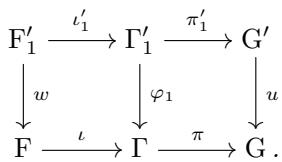
\includegraphics[keepaspectratio]{images/part002_e5b6b945.jpg}}

Then there exists a unique group homomorphism \(\psi : \Gamma_1' \to \Gamma'\) such that the diagram

\pandocbounded{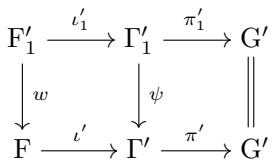
\includegraphics[keepaspectratio]{images/part002_7bcd6e81.jpg}}

commutes and \(\varphi_{1} = \varphi \circ \psi\) .

If the group homomorphism \(\psi : \Gamma_1' \to \Gamma'\) has the desired properties, then it satisfies the relations

\[
\psi (\gamma) = (\varphi \circ \psi (\gamma), \pi^ {\prime} \circ \psi (\gamma)) = (\varphi_ {1} (\gamma), \pi_ {1} ^ {\prime} (\gamma))
\]

for every \(\gamma \in \Gamma_1'\) . Conversely, the group homomorphism from \(\Gamma_1'\) to \(\Gamma \times G'\) defined by \(\gamma \mapsto (\varphi_1(\gamma), \pi_1'(\gamma))\) has values in the fiber product \(\Gamma \times_G G'\) because \(\pi \circ \varphi_1(\gamma) = u \circ \pi_1'(\gamma)\) for every \(\gamma \in \Gamma_1'\) .

COROLLARY 1. --- Let \(E_{1}\) and \(E_{2}\) be \(\tau\) -extensions of G by F, and let \(\psi\) be a morphism of \(\tau\) -extensions from \(E_{1}\) to \(E_{2}\) . Denote by \(\varphi_{1}\) (resp. \(\varphi_{2}\) ) the canonical homomorphism for \(u^{*}(\mathcal{E}_{1})\) (resp. \(u^{*}(\mathcal{E}_{2})\) ). Then there exists a unique morphism of \(\tau'\) -extensions from \(u^{*}(\mathcal{E}_{1})\) to \(u^{*}(\mathcal{E}_{2})\) , denoted by \(u^{*}(\psi)\) , such that \(\varphi_{2} \circ u^{*}(\psi) = \psi \circ \varphi_{1}\) .

It suffices to apply Proposition 1 to \(\psi \circ \varphi_{1}\) .

The class of the \(\tau^{\prime}\) -extension \(u^{*}(\mathcal{E})\) therefore depends only on the class of E. We also denote by \(u^{*}:\operatorname{Ex}_{\tau}(\mathrm{G},\mathrm{F})\to\operatorname{Ex}_{\tau^{\prime}}(\mathrm{G}^{\prime},\mathrm{F})\) the mapping that sends the class of a \(\tau\) -extension E to the class of the \(\tau^{\prime}\) -extension \(u^{*}(\mathcal{E})\) .

COROLLARY 2. --- Let \(u': G'' \to G'\) be a group homomorphism, and let \(\mathcal{E}\) be a \(\tau\) -extension of G by F. Set \(\tau'' = \tau' \circ u'\) , and denote by \(\varphi\) (resp. \(\varphi', \varphi''\) ) the canonical homomorphism associated with the \(\tau'\) -extension \(u^*(\mathcal{E})\) (resp. the \(\tau''\) -extension \(u'^*(u^*(\mathcal{E}))\) , the \(\tau''\) -extension \((u \circ u')^*(\mathcal{E})\) ). Then there exists a unique morphism \(\psi\) from the \(\tau''\) -extension \(u'^*(u^*(\mathcal{E}))\) to the \(\tau''\) -extension \((u \circ u')^*(\mathcal{E})\) such that \(\varphi'' \circ \psi = \varphi \circ \varphi'\) .

Example. --- Let H be a subgroup of G and \(j : H \to G\) the canonical injection. Then for every \(\tau\) -extension \(\mathcal{E} = (\Gamma, \iota, \pi)\) , the \(\tau \circ j\) -extension \(j^{*}(\mathcal{E})\) is isomorphic to \((\bar{\pi}^{1}(H), \iota', \pi')\) , where \(\iota' : F \to \bar{\pi}^{1}(H)\) (resp. \(\pi' : \bar{\pi}^{1}(H) \to H\) ) is the group homomorphism \(f \mapsto \iota(f)\) (resp. \(\gamma \mapsto \pi(\gamma)\) ). More generally, if the group homomorphism \(u : G' \to G\) is injective, then the canonical homomorphism \(\varphi\) is injective with image \(\bar{\pi}^{1}(u(G'))\) .
